% !TEX root = applied-math.tex




\chapter{Vector Spaces, Inner Product Spaces and Linear Transformations}

This chapter explores linear systems in a more abstract manner.  We will see that framing vector and matrix addition and scalar multiplication in a more general way will allow us to make connections between seemingly disparate parts of mathematics and then discover new things because of this.  

We first investigate vector spaces, which at first seem like they are just sets of vectors, but are actually much more.  Then we will see inner product spaces, another way of looking at vectors and finally linear transformations. 

\section{Vector Spaces}  \label{sect:vector:space}

%We start our discussion of this section with properties that we are familiar with.  We see the associative, distributive and commutative properties typically with numbers (real or complex).  Instead of restricting ourselves to only numbers, we will generalize this to what is called a field.  

%\begin{definition}
% A \textbf{field} denoted is a set together with two operations (typically called addition and multiplication), denoted $(F,+,\cdot)$ together with the following axioms:
% %
%\begin{enumerate}
% \item (closure) If $a$ and $b$ and in $F$ then $a+b$ is in $F$ and $a \cdot b$ is in $F$. 
% \item (associativity:) If $a, b,$ and $c$ are in $F$ then $(a+b)+c = a+ (b+c)$ and $(a \cdot b) \cdot c = a \cdot (b \cdot c)$.  
% \item (commutativity:) For all $a$ and $b$ in $F$, then $a+b = b+a$ and $a \cdot b = b \cdot a$. 
% \item (Additive and multiplicative identity).  There exists a number in $F$, denoted $0$ such that for all $a$ in $F$ $a+0=a$.  In addition, there exists a number denoted $1$ such that for all $a$ in $F$ that $a \cdot 1 =a$.  
% \item (existence of inverses):  For every $a$ in $F$, there exists a number $-a$ in $F$ such that $a+(-a)=0$.  In addition, there exists a number $a^{-1}$ in $F$ such that $a \cdot a^{-1}=1$. 
% \item (Distributivity):  For all $a, b$ and $c$ in $F$, $a \cdot (b +c) = a \cdot b + a \cdot c$.  
%\end{enumerate}
%\end{definition}
%
%The two fields that we are most familiar with is that of the set of reals, $\mathbb{R}$, the set of rational numbers, $\mathbb{Q}$ and the set of complex numbers, $\mathbb{C}$.  In each case, it is noted that the multiplicative inverses of 0 does not exist, however, there is a workaround for the complex numbers. 
%
%We now look at the definition of a vector space.   

A vector space as we will see is a set of vectors with a certain collection of properties.  This notion arose from vectors of $\mathbb{R}^n$, however, we will see that they generalize.  

\begin{definition} \label{def:vector:space}
Let  $V$ be a nonempty set of elements with $\vec{x}, \vec{y}, \vec{z} \in V$ and $c,k \in \mathbb{R}$.  The set $V$ is called a \textbf{real vector space} and the elements of $V$ are called \textbf{vectors} if in $V$ there are defined two algebraic operations (called \emph{vector addition}, $+$ and \emph{scalar multiplication}, $\cdot$) that satisfy the following:
 
\begin{description}
 \item[Vector Addition:] The operation $+$ satisfies:
 
\begin{enumerate}[itemindent=-0.25in]
\item (Closure):  $\vec{x}+\vec{y} \in V$.
 \item (Commutativity:)  $\vec{x} +\vec{y} = \vec{y}+\vec{x}$
 \item (Associativity:) $(\vec{x} + \vec{y}) + \vec{z} = \vec{x} + (\vec{y} + \vec{z})$ 
 \item (Identity Element:)  There exist an element $\vec{0} \in V$ that satisfies: $\vec{x} + \vec{0} = \vec{x}$.   
 \item (Inverse Elements:)  For every $\vec{x} \in V$, there exists an element denoted $-\vec{x}$ such that  $\vec{x} + (-\vec{x}) = \vec{0}$. 
\end{enumerate}

\item[Scalar Multiplication:]  The real numbers $c$ and $k$ are called \textbf{scalars}.  The operations $+$ and $\cdot$ also satisfy:
\begin{enumerate}[start=6,itemindent=-0.25in]
\item (Closure:) $c \cdot \vec{x} \in V$.  
 \item (Distributivity:) $c \cdot (\vec{x} + \vec{y}) = c\cdot  \vec{x} + c\cdot \vec{y}$
 \item (Distributivity:) $(c+k) \cdot \vec{x} = c\cdot \vec{x} + k\cdot  \vec{x}$ 
 \item (Associativity:) $c\cdot (k\cdot \vec{x}) = (ck)\cdot  \vec{x}$
 \item (Identity):  For every $\vec{x} \in V$, $1 \cdot  \vec{x} = \vec{x}$.  
\end{enumerate}
\end{description}
\end{definition}

From its name, its clear that sets of vectors are vector spaces.  We will prove this soon.  However, it is interesting that there are many other familiar sets of mathematical objects that are also vectors spaces.  We will now see these. 

\subsection{Examples of Vector Spaces}

Let's begin with the set of all vectors of length 2, which we typically write as $\mathbb{R}^2$.  

\begin{lemma} 
Show that $\mathbb{R}^2$ together with the standard notion of vector addition and scalar multiplication is a vector space. 
\end{lemma}

\begin{proof}
 Let 
 % 
\begin{align*}
 \vec{x} & = 
\begin{bmatrix}
 x_1 \\ x_2
\end{bmatrix}, & 
\vec{y} & = 
\begin{bmatrix}
 y_1 \\ y_2 
\end{bmatrix} & 
\vec{z} & = \begin{bmatrix}
z_1 \\ z_2 
\end{bmatrix}
\end{align*}
and $c,k \in \mathbb{R}$ as well as vector addition and scalar multiplication as 
% 
\begin{align*}
 \vec{x} + \vec{y} & = 
\begin{bmatrix}
 x_1 + y_1 \\ x_2 + y_2 
\end{bmatrix} & 
 c \cdot \vec{x} & = 
\begin{bmatrix}
 c x_1 \\ c x_2 
\end{bmatrix}
\end{align*}

We now show that all 10 properties of a vector space hold:
% 
\begin{enumerate}
\item (Closure) Since
%
\begin{align*}
\vec{x} + \vec{y} & = \begin{bmatrix}
x_1 \\ x_2 
\end{bmatrix} + \begin{bmatrix}
y_1 \\ y_2 
\end{bmatrix} = \begin{bmatrix}
x_1 + y_1 \\ x_2 + y_2 
\end{bmatrix}
\end{align*}
are elements of $\mathbb{R}^2$, the closure by addition holds.  

 \item (Commutativity) For all $\vec{x}, \vec{y}, \vec{z} \in V$, 
 % 
\begin{align*}
 \vec{x} + \vec{y} & = \begin{bmatrix}
 x_1 \\ x_2 
 \end{bmatrix} + \begin{bmatrix}
 y_1 \\ y_2 
 \end{bmatrix} = 
\begin{bmatrix}
 x_1 + y_1 \\ x_2 + y_2 
\end{bmatrix}\\
& =  
\begin{bmatrix}
 y_1 + x_1 \\
 y_2 + x_2 
\end{bmatrix} = \begin{bmatrix}
y_1 \\ y_2 
\end{bmatrix} + \begin{bmatrix}
x_1 \\ x_2
\end{bmatrix} = \vec{y} + \vec{x} 
\end{align*}

\item (Associativity)
\begin{align*}
 (\vec{x} + \vec{y}) + \vec{z} & = 
\biggl( \begin{bmatrix}
 x_1 \\ x_2
 \end{bmatrix} + \begin{bmatrix}
 y_1 \\ y_2 
 \end{bmatrix} \biggr) + \begin{bmatrix}
 z_1 \\ z_2
 \end{bmatrix} \\
 & = 
\begin{bmatrix}
 x_1 + y_1 \\
 x_2 + y_2 
\end{bmatrix} + \begin{bmatrix}
z_1 \\ z_2 
\end{bmatrix} \\
& = 
\begin{bmatrix}
 (x_1 + y_1) + z_1 \\
 (x_2 + y_2) + z_2 
\end{bmatrix} \\
& =
\begin{bmatrix}
 x_1 + (y_1 + z_1) \\
 x_2 + (y_2 + z_2)
\end{bmatrix} 
= \begin{bmatrix}
x_1 \\ x_2
\end{bmatrix}+ 
\begin{bmatrix}
 y_1 + z_1 \\
 y_2 + z_2 
\end{bmatrix}\\
 &  = \begin{bmatrix}
x_1 \\ x_2 
\end{bmatrix} + \biggl( \begin{bmatrix}
y_1 \\ y_2 
\end{bmatrix} + \begin{bmatrix}
z_1 \\ z_2 
\end{bmatrix} \biggr) = \vec{x} + (\vec{y} + \vec{z}) 
\end{align*}

\item (Identity Element)  The zero element $\vec{0}$ is 
% 
\begin{align*}
 \vec{0} & = 
\begin{bmatrix}
 0 \\ 0 
\end{bmatrix}
\end{align*}
%
and it satisfies,
%
\begin{align*}
 \vec{0} + \vec{x} & = 
\begin{bmatrix}
 0 \\ 0 
\end{bmatrix} + 
\begin{bmatrix}
 x_1 \\ x_2 
\end{bmatrix} = 
\begin{bmatrix}
 0 + x_1 \\ 0 + x_2 
\end{bmatrix} = 
\begin{bmatrix}
 x_1 \\ x_2 
\end{bmatrix} = \vec{x} 
\end{align*}

\item (Inverse Element) The inverse element $-\vec{x}$ is given as 
% 
\begin{align*}
 -\vec{x} & = 
\begin{bmatrix}
 -x_1 \\ -x_2
\end{bmatrix}
\end{align*}
%
and the following satisfies:
% 
\begin{align*}
 \vec{x} + (-\vec{x}) & = 
\begin{bmatrix}
 x_1 \\ x_2 
\end{bmatrix} + 
\begin{bmatrix}
 -x_1 \\ -x_2 
\end{bmatrix}
= 
\begin{bmatrix}
 x_1 + (-x_1) \\ x_2 + (-x_2) 
\end{bmatrix} = 
\begin{bmatrix}
 0 \\ 0 
\end{bmatrix} = \vec{0} 
\end{align*}

\item (Closure) ~~ For $c \in \mathbb{R}$, 
%
\begin{align*}
c \cdot \vec{x} & = c \cdot  \begin{bmatrix}
x_1 \\ x_2 
\end{bmatrix} = \begin{bmatrix}
cx_1 \\ cx_2 
\end{bmatrix}
\end{align*}
which is in $\mathbb{R}^2$, so scalar multiplication is closed.  

\item (Distributivity) 
 ~~ Let $c \in \mathbb{R}$ and 
% 
\begin{align*}
 c \cdot (\vec{x} + \vec{y}) & = 
 c \cdot \biggl( 
\begin{bmatrix}
 x_1 \\ x_2 
\end{bmatrix} + 
\begin{bmatrix}
 y_1 \\ y_2 
\end{bmatrix} \biggr) 
= c\cdot 
\begin{bmatrix}
 x_1 + y_1 \\
 x_2 + y_2 
\end{bmatrix} 
= 
\begin{bmatrix}
 c (x_1 +y_1) \\ c (x_2 + y_2) 
\end{bmatrix} \\
& = 
\begin{bmatrix}
 c x_1 + c y_1 \\
 c x_2 + c y_2 
\end{bmatrix} 
= 
\begin{bmatrix}
 c x_1 \\ c x_2 
\end{bmatrix} + 
\begin{bmatrix}
 c y_1 \\ c y_2 
\end{bmatrix} 
= c \cdot 
\begin{bmatrix}
 x_1 \\ x_2 
\end{bmatrix}
+ c \cdot 
\begin{bmatrix}
 y_1 \\ y_2 
\end{bmatrix} \\
& = c\cdot  \vec{x} + c\cdot  \vec{y} 
\end{align*}

\item (Distributivity)~~  Let $c$ and $k$ be elements of $\mathbb{R}$. 
%
\begin{align*}
 (c + k)\cdot  \vec{x} & = (c+k) \cdot 
\begin{bmatrix}
 x_1 \\ x_2 
\end{bmatrix} = 
\begin{bmatrix}
 (c+k) x_1 \\ (c+k) x_2 
\end{bmatrix} = 
\begin{bmatrix}
 c x_1 + k x_1 \\
 c x_2 + k x_2 
\end{bmatrix} \\
& = 
\begin{bmatrix}
 c  x_1 \\ c x_2 
\end{bmatrix} + 
\begin{bmatrix}
 k x_1 \\ k x_2 
\end{bmatrix} = c \cdot 
\begin{bmatrix}
 x_1 \\ x_2 
\end{bmatrix} + k \cdot 
\begin{bmatrix}
 x_1 \\ x_2 
\end{bmatrix} = c \cdot \vec{x} + k \cdot \vec{x} 
\end{align*}

\item (Associativity) ~~ Let $c$ and $k$ be elements of $\mathbb{R}$. 

\begin{align*}
 c\cdot (k\cdot \vec{x}) & = c \cdot \biggl( k \cdot 
\begin{bmatrix}
 x_1 \\ x_2 
\end{bmatrix} \biggr) = c \cdot 
\begin{bmatrix}
 k x_1 \\ k x_2 
\end{bmatrix} = 
\begin{bmatrix}
 c (k x_1) \\ c (kx_2) 
\end{bmatrix} = 
\begin{bmatrix}
 (c k) x_1 \\ (ck) x_2 
\end{bmatrix} \\
& = (ck) \cdot 
\begin{bmatrix}
 x_1 \\ x_2 
\end{bmatrix} = (ck) \cdot \vec{x} 
\end{align*}

\item (Identity element)

\begin{align*}
1 \cdot \vec{x} & = 1\cdot  \begin{bmatrix}
x_1 \\ x_2 
\end{bmatrix} = \begin{bmatrix}
x_1 \\ x_2 
\end{bmatrix} = \vec{x}
\end{align*}

\end{enumerate}
\end{proof}


The following are also vector spaces.  There are not proofs associated with these.  

\begin{itemize}
 
 \item The set of vectors that consist of  $\mathbb{R}^3$ with the standard definition of vector addition and scalar multiplication. 
 \item The set of vectors that consist of  $\mathbb{R}^n$ with the standard definition of vector addition and scalar multiplication. 
\item The set of all $m \times n$ matrices, $\mathcal{M}_{m \times n}$ with standard definition of matrix addition and scalar multiplication. 

\end{itemize}

In the next few examples, we will also show some other interesting sets are vector spaces.  To save a bunch of time and effort, in some cases, we don't need to show all 10 properties.  We can skip most of properties, if the set $V$ is a subset of a known vector space.  

The reason for this is that properties 2--5 and 7--10 will automatically hold because the vectors are already in a vector space.  We will do this formally in the next section.  


\begin{example} \label{ex:lines:through:origin:vector:space}

Show that all lines that pass through the origin, or the set
%
\begin{align*}
V & = \{ ax + by = 0\; | \; x, y \in \mathbb{R} \text{~ and both $a$ and $b$ are not both 0.} \} 
\end{align*}
%
is a vector space. 

\solution

First, let's rewrite the vector space as 
\begin{align*}
V & = \{ \begin{bmatrix}
u_1 \\ u_2 
\end{bmatrix} \; | \; \text{$au_1+bu_2=0$, with $a$ and $b$ both not 0.}\}
\end{align*}
because this is the same set of points, but it is written in terms of a vector, which makes things easier to show. 

As stated above, since $V$ is a subset of $\mathbb{R}^2$, we don't need to prove properties 2--5, 7--10, which hold because we already showed that these properties show.  Instead, to save time and effort, we only prove properties 1 and 6 of definition of a vector space in Definition \ref{def:vector:space}.  

\begin{enumerate}
\item Let $\vec{u}, \vec{v} \in V$.  Therefore the two equations $au_1+bu_2=0$ and $av_1+bv_2=0$ are satisfied.  Now check the sum, 
%
\begin{align*}
\vec{u} + \vec{v} & = \begin{bmatrix}
u_1 + v_1 \\
u_2 + v_2 
\end{bmatrix}
\end{align*}
and need to show that this is in $V$.  Since 
\begin{align*}
a(u_1 + v_1) + b(u_2+v_2) & = au_1 + av_1 + bu_2 + bv_2  \\
& = 
(au_1 + bu_2) + (av_1 + bv_2) = 0 + 0 = 0
\end{align*}
then $\vec{u}+\vec{v} \in V$.  

\setcounter{enumi}{5}

\item We need to show that $r \cdot \vec{u} \in V$, so that the vector $r\cdot\vec{u}$ satisfies the property that the line passes through the origin.  
%
\begin{align*}
r \cdot \vec{u} & = \begin{bmatrix}
r u_1 \\ r u_2 
\end{bmatrix}
\end{align*}
and since $au_1 + bu_2 = 0$, then 
\begin{align*}
r \cdot 0  = r(au_1 + bu_2) & = a (ru_1) + b (r u_2)  =0 
\end{align*}
therefore $r \cdot \vec{u} \in V$.  
\end{enumerate}
So this is a vector space.  


\end{example}

The next example shows that polynomials (specifically quadratics) are vector spaces.  Since we haven't shown anything about polynomials yet, we need to show all 10 properties of Definition \ref{def:vector:space} hold.  

\begin{example}
Show than the set, $\mathcal{P}_2$, the set of all polynomials of degree $2$ is a vector space with vector addition defined as the sum of two polynomials and scalar multiplication as the multiplication of a polynomial by a constant.  

\solution


In this case scalars are elements in $\mathbb{R}$ and the vector space $V$ is the set of all polynomials of degree at most $2$.   Let 
  % 
\begin{align*}
 \vec{x} & = a_0 + a_1 x + a_2 x^2 \\
 \vec{y} & = b_0 + b_1 x + b_2 x^2 \\
 \vec{z} & = c_0 + c_1 x + c_2 x^2 
\end{align*}
  
Vector addition is simply polynomial addition for example:
%
\begin{align*}
\vec{x} + \vec{y} & = (a_0 + a_1 x + a_2 x^2) + (b_0 + b_1 x + b_2 x^2) \\
& = (a_0 + b_0) + (a_1 + b_1) x + (a_2 + b_2) x^2.  
\end{align*}
and scalar addition is given by 
%
\begin{align*}
r \vec{x} & = r(a_0 + a_1 x + a_2 x^2) = (ra_0) + (ra_1) x + (ra_2) x^2
\end{align*}  
  
\begin{enumerate}
\item (Closure)~~ Show that $\vec{x}+\vec{y}$ is in $\mathcal{P}_2$, the set of polynomials of degree 2. 
\begin{align*}
\vec{x} + \vec{y} & = (a_0 + a_1 x + a_2 x^2) + (b_0 + b_1 x+ b_2 x^2) \\
& = (a_0 + b_0) + (a_1 + b_1) x + (a_2 + b_2) x^2 
\end{align*}
which is a polynomial of degree 2, so this is in $\mathcal{P}_2$. 

 \item (Commutativity)  
\begin{align*}
 \vec{x} + \vec{y} & = (a_0 + a_1 x + a_2 x^2) + (b_0 + b_1 x +b_2 x^2) \\
 & = (b_0 + b_1 x + b_2 x^2) + (a_0 + a_1 x +  a_2 x^2) \\
 & = \vec{y} + \vec{x} 
\end{align*}

\item (Associativity)
\begin{align*}
 (\vec{x} + \vec{y}) + \vec{z} & = (a_0 + a_1 x + a_2 x^2+ b_0 + b_1 x + b_2 x^2) \\
 & \qquad+ (c_0 + c_1 x + c_2 x^2) \\
 & = a_0 + a_1 x + a_2 x^2 \\
 & \qquad + (b_0 + b_1 x + b_2 x^2) + (c_0 + c_1 x + c_2 x^2) \\
 & = \vec{x} + (\vec{y} + \vec{z}) 
\end{align*} 

\item (Additive Identity) ~~The zero element $\vec{0}$ is the function 0.  
% 
\begin{align*}
 \vec{0} + \vec{x} & = 0 + a_0 + a_1 x + a_2 x^2 \\
 & = a_0 + a_1 x + a_2 x^2 = \vec{x} 
\end{align*}

\item (Additive Inverse)~~The inverse element $-\vec{x}$ is $-a_0 - a_1 x-a_2x^2$, and 
\begin{align*}
\vec{x} + (-\vec{x}) & = (a_0 + a_1 x + a_2 x^2) + (-a_0 - a_1 x-a_2x^2) \\
& = (a_0 -a_0) + (a_1 -a_1) x + (a_2 -a_2) x^2 = 0 = \vec{0}. 
\end{align*}

\item (Closure under scalar multiplication)
\begin{align*}
r \vec{x} & = r(a_0 + a_1 x + a_2 x^2) = (ra_0) + (ra_1) x + (ra_2) x^2
\end{align*}
since this is a polynomial of degree 2, then $r \vec{x} \in \mathcal{P}_2$.  

\item (Distributivity) ~~Let $r, s \in \mathbb{R}$, 
%
\begin{align*}
(r + s) \vec{x} & = (r+s) (a_0 + a_1 x + a_2 x^2) \\
& = r (a_0 + a_1 x + a_2 x^2) + s (a_0 + a_1 x + a_2 x^2) = r \vec{x} + s \vec{x}
\end{align*}

\item (Distributivity) ~~Let $r \in \mathbb{R}$, 
%
\begin{align*}
r (\vec{x} + \vec{y}) & = r ((a_0 + a_1 x + a_2 x^2) + (b_0 + b_1 x + b_2 x^2)) \\
& =r (a_0 + a_1 x + a_2 x^2) + r (b_0 + b_1 x + b_2 x_2)  \\
& = r \vec{x} + r \vec{y} 
\end{align*}

\item (Associativity)~~ Let $r, s \in \mathbb{R}$, 
\begin{align*}
(rs) \vec{x} & = (rs) (a_0 + a_1 x + a_2 x^2) = r (s(a_0 + a_1 x + a_2 x^2)) \\
& = r (s \vec{x}) 
\end{align*}

\item (Multiplicative Identity)
\begin{align*}
1 \cdot \vec{x} & = 1 (a_0 + a_1 x + a_2 x^2) = a_0 + a_1 x + a_2 x^2 = \vec{x}.  
\end{align*}
\end{enumerate}
  \end{example} 

The above example shows that there are examples of vectors and vector spaces that don't seem like vectors in $\mathbb{R}^n$.  The following are also vector spaces:
\begin{itemize}
  \item The set $\{a \sin x + b \cos x \; | \; a, b \in \mathbb{R} \}$. 
  \item The set $\{ f \; | \; f: \mathbb{R} \rightarrow \mathbb{R} \}$ of functions of a single variable.  

The ``vector addition'' is given by $(f+g) (x)= f(x) + g(x)$ and the ``scalar multiplication'' is $(r \cdot f) (x) = r \cdot f(x)$.  

We won't cover all of the properties of this set mainly because the real-valued function derive their properties from the reals, which is a vector space.  


\item The set of functions that satisfy $f'+f=0$.  
  \item Solutions of homogeneous differential equations, which is a generalization of functions that satisfy $f'+f=0$.    
\end{itemize}

\subsubsection{Is every set a vector space?}

In short, no.  For example, consider the following:

%
\begin{align*}
V = \{ \begin{bmatrix}
x_1 \\ x_2 
\end{bmatrix} \; | \; x_1 \geq 0, x_2 \geq 0 \} 
\end{align*}
which is the first quadrant of the plane.     To check if this is a vector space, we don't need to check all 10 properties.  This is because since $V$ is a subset of $\mathbb{R}^2$, most of the properties (commutative, associative, distributive, for examples) will work just as they did in $\mathbb{R}^2$.  The only two that we do need to check are the closure properties.  

\begin{enumerate}
\item If $\vec{u}, \vec{v} \in V$, then 
%
\begin{align*}
\vec{u} + \vec{v} & = \begin{bmatrix}
u_1 + v_1 \\
u_2 + v_2 
\end{bmatrix}
\end{align*}
and since $u_1, u_2, v_1, v_2$ all satisfy $\geq 0$, then this vector is in $V$. 

\setcounter{enumi}{5}

\item Let $r \in \mathbb{R}$, then 
%
\begin{align*}
r \vec{u} & = \begin{bmatrix}
r u_1 \\ r u_2
\end{bmatrix}
\end{align*}
but if $r<0$ then $r \vec{u} \not \in V$, so $V$ is not a vector space.  
\end{enumerate}


\begin{example}
Is the set $\displaystyle U=\{ \begin{bmatrix}
x_1 \\ x_2 
\end{bmatrix} \; | \; x_1^2+x_2^2=1\}$ a vector space?  If not what properties does it violate?  

\solution

This set is a circle of radius one centered at the origin.  Again, like above, $U$ is a subset of $\mathbb{R}^2$ and thus the properties to check are the closure properties.  

\begin{enumerate}
\item If we let 
%
\begin{align*}
\vec{x} &= \begin{bmatrix}
x_1 \\ x_2 
\end{bmatrix}& \vec{y} & = \begin{bmatrix}
y_1 \\ y_2 
\end{bmatrix}
\end{align*}
both be in $U$, then 
%
\begin{align*}
\vec{x}+\vec{y} & = \begin{bmatrix}
x_1 + y_1 \\ x_2 +y_2 
\end{bmatrix}
\end{align*}
Is this in $U$.  To check sum the squares of the individual elements. 
%
\begin{align*}
(x_1+y_1)^2 + (x_2+y_2)^2 & = x_1^2+ 2x_1y_1 + y_1^2+x_2^2+ 2x_2y_2 + y_1^2 \\
& = 2 + 2x_1y_1 + 2 x_2 y_2 
\end{align*}
which is only 1 in special circumstances and not in general, so this is not a vector space. 

\setcounter{enumi}{3}
\item The additive identity requires that the zero vector is an element of the vector space.  However, since
%
\begin{align*}
\begin{bmatrix}
0 \\ 0
\end{bmatrix} 
\end{align*}
is not in $U$, then this property is also not satisfied. 

\setcounter{enumi}{5}
\item This property is also not satisfied for the same reason as \#1.  Geometrically if $\vec{x}$ is in $U$ then $r\vec{x}$ is on a circle of radius $r$, so won't be in $U$ in general.  
\end{enumerate}

\end{example}



\section{The Span and Basis of a Subspace}

In section \ref{sect:linear:comb:span}, we saw the span of vectors in $\mathbb{R}^n$.  We now extend this example to the span of any subspace.  In addition, the notion of a basis  of the subspace is introduced.  

\begin{definition}
For any vector space, $V$ a \textbf{subspace}, $U$ is a subset of $V$ that itself is a vector space.  
\end{definition}

\begin{example}
We showed in example \ref{ex:lines:through:origin:vector:space} that the set of all lines in $\mathbb{R}^2$ that pass through the origin is a vector space.  Since the set is a subset of $\mathbb{R}^2$, it is a subspace of $\mathbb{R}^2$ as well. 
\end{example}


\begin{example}
Show that $\mathbb{R}^2$ is a subspace of $\mathbb{R}^3$.  

\solution

Since $\mathbb{R}^2$ is itself a vector space and a subset of $\mathbb{R}^3$, then $\mathbb{R}^2$ is a subspace. 
\end{example}



\begin{example}
Recall that the set
  \begin{align*}
{\cal P}_2=\{ a_0 + a_1 x + a_2 x^2\; | \; a_0, a_1, a_2 \in \mathbb{R} \}
 \end{align*}
is the set of all quadratic functions.  

The set ${\cal P}_1 = \{a_0 + a_1 x \; | \; a_0, a_1 \in \mathbb{R} \}$ of all linear functions is itself a vector space as well as a subset of ${\cal P}_2$, therefore ${\cal P}_1$ is a subspace of ${\cal P}_2$.

In addition, the set $\{ a x^2\; | \; a \in \mathbb{R}\}$ is a vector space as well as a subset of ${\cal P}_2$, therefore it is a subspace.  
\end{example}

The above examples show that there are many already known subspaces.  There are many cases though that aren't evident or to show it is a subspace, we would need to prove all 10 properties that it is a vector space.  The next lemma, however, shows that isn't the case.  

\begin{lemma}
Let $S$ be a nonempty subset $S$ of a vector space $V$, under the inherited operations. 
If for all $\vec{s}_1$ and $\vec{s}_2$ in $S$ and $r_1, r_2 \in \mathbb{R}$ 
%
\begin{align*}
r_1 \vec{s}_1 + r_2 \vec{s}_2 \in S
\end{align*}
then $S$ is a subspace. 

\label{lemma:subspace}
\end{lemma}

This means that if $S$ is a subset of $V$, that we know is a vector space, to prove that $S$ is a subspace, we only need to check if $r_1 \vec{s}_1 + r_2 \vec{s}_2 \in S$. 


\begin{proof}
Since $S$ is a subspace of $V$, properties (2)--(5) and (7)--(10) of Definition \ref{def:vector:space} hold for $S$.  Thus we only need to prove closure under addition and scalar multiplication. 

Property 1:  Because $r_1 \vec{s}_1 + r_2 \vec{s}_2 \in S$, let $r_1=r_2=1$, thus $\vec{s}_1+\vec{s}_2 \in S$. 

Property 6: Because $r_1 \vec{s}_1 + r_2 \vec{s}_2 \in S$, let $r_2=0$, thus $r_1 \vec{s}_1 \in S$.  

\end{proof}


\begin{example}
 Show that
 %
 \begin{align*}
 V & = \{ \begin{bmatrix}
 v_1 \\ v_2 
 \end{bmatrix} \; | \; v_2 = k v_1 \}
 \end{align*}
(that is, all vectors on a line of slope $k$) is a subspace of $\mathbb{R}^2$. 
 
 \solution
 
 We will use lemma \ref{lemma:subspace}.  Let 
%
\begin{align*}
\vec{u} & = \begin{bmatrix}
u_1 \\ u_2 
\end{bmatrix} & \vec{v} & = \begin{bmatrix}
v_1 \\ v_2 
\end{bmatrix}
\end{align*}
be elements of $V$.  That is $v_2 = k v_1$ and $u_2 = ku_1$.  Then 
%
\begin{align*}
r_1 \vec{u} + r_2 \vec{v} & = r_1 \begin{bmatrix}
u_1 \\ k u_1 
\end{bmatrix} + r_2 \begin{bmatrix}
v_1 \\ k v_1 
\end{bmatrix} =  \begin{bmatrix}
r_1 u_1 + r_2 v_1 \\ r_1 k u_1 + r_2 k v_1 
\end{bmatrix} \\
& = \begin{bmatrix}
r_1 u_1 + r_2 v_1 \\ k (r_1 u_1 + r_2 v_1) 
\end{bmatrix}
\end{align*}
which is an element of $V$ because the second component is $k$ times the first one. Thus $V$ is a subspace of $\mathbb{R}^2$.  
\end{example}

\phantom{hi}

\begin{example}  \label{eq:example:diag:matrix}
Show using Lemma \ref{lemma:subspace} that 
%
\begin{align*}
V& =\{ \begin{bmatrix}
a & 0 \\
0 & b 
\end{bmatrix} \; | \; a,b \in \mathbb{R} \}
\end{align*}
the set of all diagonal matrices is a subspace of ${\cal M}_{2 \times 2}$.  

\solution 

In this case, if we show that for any two matrices
\begin{align*}
A & = \begin{bmatrix}
a_1 & 0 \\
0 & b_1 
\end{bmatrix}, & B & = \begin{bmatrix}
a_2 & 0 \\
0 & b_2
\end{bmatrix} 
\end{align*} and scalars $r_1, r_2 \in \mathbb{R}$ that  $r_1 A + r_2 B$ is in the set. 

\begin{align*}
r_1 A + r_2 B & = r_1 \begin{bmatrix}
a_1 & 0 \\
0 & b_1 
\end{bmatrix}+ r_2 \begin{bmatrix}
a_2 & 0 \\
0 & b_2
\end{bmatrix} \\
& = \begin{bmatrix}
r_1 a_1 + r_2 a_2 & 0 \\
0 & r_1 b_1 + r_2 b_2 
\end{bmatrix}
\end{align*} 
which is a diagonal matrix, therefore in $V$, thus this is a subspace.  
\end{example}

\begin{lemma}
Let $A$ be an $m$ by $n$ matrix.  The null space of $A$ is a subspace of $\mathbb{R}^n$.  

\end{lemma}


\begin{proof}

We will use lemma \ref{lemma:subspace} to solve this. Let both $\vec{x}$ and $\vec{y}$ be in the null space of $A$.  This means that $A\vec{x}=\vec{0}$ and $A\vec{y}=\vec{0}$.   We need to show that $r_1 \vec{x} + r_2 \vec{y}$ is in the null space of $A$. 


\begin{align*}
A(r_1 \vec{x} + r_2 \vec{y}) & = r_1 A\vec{x} + r_2 A\vec{y} \\
& = r_1 (0) + r_2 (0) = 0 
\end{align*}
Vectors in the null space are vectors of length $n$, so the null space is a subset of $\mathbb{R}^n$ and since  $r_1 \vec{x} + r_2 \vec{y}$ is in the null space of $A$, then the null space is a subspace of $\mathbb{R}^n$.  

\end{proof}

This is an important result that we will see in eigenvalues in the next chapter.  




\subsection{The Span of a set of vectors}


We saw in  Section \ref{sect:linear:comb:span} the span of a set of vectors in $\mathbb{R}^n$.  We now generalize this to any vector space.  

\begin{definition}
The \textbf{span} of a nonempty set subset $S$ of a vector space is the set of all linear combinations of the vectors in $S$.  
%
\begin{align*}
\text{span}(S) & = \{ c_1 \vec{s}_1 + c_2 \vec{s}_2 + \cdots + c_n \vec{s}_n\; | \; \text{$c_1, c_2, \ldots, c_n \in \mathbb{R}$, $\vec{s}_1, \vec{s}_2, \ldots, \vec{s}_n \in S$} \}.  
\end{align*}
\end{definition}

To show that a subset of vectors span a subspace $S$, we need to show that any vector in $S$ can be written as a linear combination of the spanning vectors.  

\begin{example}
Show that the set $\{2+x,1,x+x^2\}$ spans $\mathcal{P}_2$.  

\solution
In this case, we need show that a general polynomial in $\mathcal{P}_2$ can be written as a linear combination of elements of the given set.  That is
%
\begin{align*}
c_1 (2+x) + c_2 (1) + c_3 (x+x^2) = a_0 + a_1 x + a_2 x^2 
\end{align*}
and if there is a solution for the $c$'s, then that shows the the set spans $\mathcal{P}_2$.  To find the solution, use the technique of equating coefficients. Write down the coefficients for the constant terms, $x$ terms and $x^2$ terms respectively. 
%
\begin{align*}
2 c_1 + c_2 & = a_0 \\
c_1 + c_3 & = a_1 \\
c_3 & = a_2 
\end{align*}
This has a solution $c_3=a_2, c_1 = a_1-a_2$ and $c_2 = a_0 - 2(a_1-a_2)$, so the given set spans $\mathcal{P}_2$.  

\end{example}


\begin{lemma}
The span of any subset of a vector space is a subspace.  
\end{lemma}

\begin{proof}
Let $S$ be the subset and $\vec{s}_1, \vec{s}_2, \ldots, \vec{s}_n$ be the elements of $S$.   Using Lemma \ref{lemma:subspace}, we need to check that $\text{span}(S)$ is closed under linear combinations.  Let
%
\begin{align*}
\vec{v} & = c_1 \vec{s}_1 + c_2 \vec{s}_2 + \cdots + c_n \vec{s}_n, \\
\vec{w} & = k_1 \vec{s}_1 + k_2 \vec{s}_2 + \cdots + k_n \vec{s}_n
\end{align*}
then 
\begin{align*}
r_1 \vec{v} + r_2 \vec{w} & = r_1 (c_1 \vec{s}_1 + c_2 \vec{s}_2 + \cdots + c_n \vec{s}_n) + 
r_2 (k_1 \vec{s}_1 + k_2 \vec{s}_2 + \cdots + k_n \vec{s}_n) \\
& = (r_1 c_1 + r_2 k_1) \vec{s}_1 + (r_1c_2 + r_2 k_2) \vec{s}_2 + \cdots + (r_1 c_n + r_2 k_n) \vec{s}_n 
\end{align*}

Since this shows that $r_1 \vec{v} + r_2 \vec{w}$ is in $S$, then $S$ is a subspace.  
\end{proof}

This lemma allows us to talk about a vector space in terms of the vectors that span it.  For example, instead of thinking of $\mathcal{P}_2$, we think of the span of $\{2+x,1,x+x^2\}$ (in this case, it may not be more helpful, but other cases it is).  

\begin{example}
 Show that the following vectors span $\mathbb{R}^3$:
 % 
\begin{align*}
 \vec{e}_1 & = 
\begin{bmatrix}
 1 \\ 0 \\ 0 
\end{bmatrix}, & \vec{e}_2 & = 
\begin{bmatrix}
 0 \\ 1 \\ 0 
\end{bmatrix}, & \vec{e}_3 & = 
\begin{bmatrix}
 0 \\ 0 \\ 1
\end{bmatrix}
\end{align*}

\solution 

Because the vector $\vec{x}=[x_1,x_2,x_3]^T$ can be written $\vec{x}=x_1 \vec{e}_1 + x_2 \vec{e}_2 + x_3 \vec{e}_3$, then these vectors span $\mathbb{R}^3$.  
\end{example}


\begin{example}
Does $\{2+x,x^2 \}$ span $\mathcal{P}_2$?  

\solution 

To determine this, we will try write a general polynomial in $\mathcal{P}_2$, 
%
\begin{align*}
a_0 + a_1 x + a_2 x^2
\end{align*}
in term of the set or 
%
\begin{align*}
a_0 + a_1 x + a_2 x^2 & = c_1 (2+x) + c_2 x^2
\end{align*}
and equating coefficients, 
%
\begin{align*}
a_0 & = 2c_1  \\
a_1 & = c_1 \\
a_2 & = c_2
\end{align*}

There's no solution to this because $c_1$ can't simultaneously equal $a_1$ and $a_0/2$, so  $\{2+x,x^2\}$ does not span $\mathcal{P}_2$.  
\end{example}


\subsection{The Basis and Dimension of a Vector Space}

\begin{definition}
The \textbf{basis} of a vector space is a sequence of vectors of the vector space that form a linearly independent set that spans the vector space.  
\end{definition}

Note: the basis will be a sequence of vectors because the order of the vectors will be important.  We will denote the sequence with parentheses, $( \vec{s}_1, \vec{s}_2, \ldots )$.  


\begin{example}
We showed in Example \ref{ex:span:2} that the set $\displaystyle
\{ \begin{bmatrix}
1 \\ 0
\end{bmatrix}, \begin{bmatrix}
1 \\1 
\end{bmatrix} \} $ 
span $\mathbb{R}^2$ and since the second is not a multiple of the first, they are linearly independent.  Therefore the sequence
%
\begin{align*}
( \begin{bmatrix}
1 \\ 0
\end{bmatrix}, \begin{bmatrix}
1 \\1 
\end{bmatrix} )
\end{align*}
form a basis for $\mathbb{R}^2$.  
\end{example}

\begin{example}
The sequence of vectors \begin{align*}
( \begin{bmatrix}
1 \\ 1
\end{bmatrix}, \begin{bmatrix}
1 \\0 
\end{bmatrix} )
\end{align*}
is a different basis of $\mathbb{R}^2$ because of the order of vectors.  The fact that they span $\mathbb{R}^2$ and are linearly independent do not depend on the order. 
\end{example}

\phantom{hi}

\begin{example}
There are many bases of a vector space.  For example, 
%
\begin{align*}
( \begin{bmatrix}
1 \\ 0
\end{bmatrix}, \begin{bmatrix}
0 \\1 
\end{bmatrix} )
\end{align*}
also spans $\mathbb{R}^2$ and are linearly independent.  
\end{example}

\phantom{hi}

\begin{example}
Does
\begin{align*}
( \begin{bmatrix}
1 \\ 0
\end{bmatrix}, \begin{bmatrix}
1 \\1 
\end{bmatrix},
\begin{bmatrix}
2 \\ 3
\end{bmatrix} )
\end{align*}
form a basis of $\mathbb{R}^2$?  

\solution

These three vectors are not linearly independent.  Although one can show this in general, note that
%
\begin{align*}
\begin{bmatrix}
2 \\ 3
\end{bmatrix} & = 3 \begin{bmatrix}
1 \\ 1
\end{bmatrix} - \begin{bmatrix}
1 \\ 0 
\end{bmatrix}
\end{align*}
and since they are not linearly independent, then they cannot form a basis of $\mathbb{R}^2$.  

\end{example}

Although there are lots of different bases for a given subspace, there are some that are more useful than others.  There is a basis for more subspaces called a standard basis.  


\begin{definition}
The sequence
%
\begin{align*}
{\cal E}_n & = (
\begin{bmatrix}
1 \\ 0 \\ 0 \\ \vdots \\ 0
\end{bmatrix}, \begin{bmatrix}
0 \\ 1 \\ 0 \\ \vdots \\ 0
\end{bmatrix}, \cdots 
\begin{bmatrix}
0 \\ 0 \\ 0 \\ \vdots \\ 1
\end{bmatrix} )
\end{align*}
is called the \textbf{standard basis} or \textbf{natural basis} of $\mathbb{R}^n$.  The vectors in the basis are called $\vec{e}_1, \vec{e}_2, \ldots$. 
\end{definition}

\begin{Boxed*}
The natural basis of ${\cal P}_3$ is $( 1, x, x^2, x^3 )$.  
\end{Boxed*}

We saw bases of vector spaces (or subspaces) at the beginning of this course.  In Example \ref{ex:large:linear:solution}, we solved a linear system.  It's associated homogeneous system is 
%
\begin{align*}
x_2 + 3x_3 -9 x_4 + 11 x_5 & = 0, \\
2x_3 \phantom{-9x_4} + 4x_5 & = 0, \\
3x_5 & = 0, 
\end{align*}

The solution (which is a subspace of $\mathbb{R}^5$) can be written as
%
\begin{align*}
\{\begin{bmatrix}
1 \\ 0 \\ 0 \\ 0 \\ 0 
\end{bmatrix} x_1 + \begin{bmatrix}
0 \\ 9 \\ 0 \\ 1 \\ 0
\end{bmatrix} x_4 \; | \; x_1, x_4 \in \mathbb{R}, \} 
\end{align*}

The two vectors in the solution are a basis of the solution space.  Since there are only two vectors and they are not constant multiples of each other, it's easy to see that they are linearly independent.  Also because of the form of the solution set, you can also see that that span the space.  

\begin{definition}
In a vector space with basis $B$, the \textbf{representation of a vector $\vec{v}$ with respect to the basis $B$} is the column vector of the coefficients used to express $\vec{v}$ as a linear combination of the basis vectors:
%
\begin{align*}
\text{Rep}_B (\vec{v}) & = \begin{bmatrix}
c_1 \\ c_2 \\ \vdots \\ c_n 
\end{bmatrix}
\end{align*}
where $B=( \vec{\beta}_1, \vec{\beta}_2, \ldots , \vec{\beta}_n )$ and
%
\begin{align*}
\vec{v} & = c_1 \vec{\beta}_1 + c_2 \vec{\beta}_2 + \cdots + c_n \vec{\beta}_n
\end{align*}
\end{definition}

\begin{example}
Consider the space ${\cal P}_2$, the space of quadratic functions.  Let $B=( 1, 1+x,1+x+x^2, )$ be a basis of ${\cal P}_2$ and $\vec{v} = 2x+x^2$.  To find the representation, we need to find $c_1, c_2$ and $c_3$ such that
%
\begin{align*}
c_1 \cdot 1 + c_2 \cdot (1+x) + c_3 \cdot (1+x+x^2) & = 2x+x^2
\end{align*}
by equating coefficients this is same as solving the linear system:
%
\begin{align*}
c_1 + c_2 + c_3 & = 0 \\
c_2 + c_3 & = 2 \\
c_3  & = 1
\end{align*}
resulting in $c_1=-2, c_2=1, c_3=1$, therefore
%
\begin{align*}
\text{Rep}_B (\vec{v}) & = \begin{bmatrix}
-2 \\ 1 \\ 1
\end{bmatrix}
\end{align*}

If instead the basis is given as $D=( 2,2x,x^2 )$, then 
%
\begin{align*}
\text{Rep}_D (\vec{v})& = \begin{bmatrix}
0 \\ 1 \\ 1
\end{bmatrix}
\end{align*}
\end{example}


\subsubsection{Representations in the natural basis}

As we saw above, finding representations in a basis requires solving another linear system.  However, representations in the natural basis are simple calculations.  If we used the natural basis $E=( 1, x, x^2 )$ for the quadratic example above, then 
%
\begin{align*}
\text{Rep}_E (\vec{v}) & = \begin{bmatrix}
0 \\ 2 \\ 1
\end{bmatrix}
\end{align*}
are just the coefficients of $x^n$ terms of the vector $2x+x^2$.   The following example shows that the representation of a vector in $\mathbb{R}^3$ is what we expect, itself. 

\vspace{0.5in}

~ 

\begin{example}
Find the Representation of the vector
%
\begin{align*}
\vec{v} & = \begin{bmatrix}
-3 \\ 2\\ 4 
\end{bmatrix}
\end{align*}
in the natural basis
%
\begin{align*}
{\cal E}_3 & = (
\begin{bmatrix}
1 \\ 0 \\ 0
\end{bmatrix}, \begin{bmatrix}
0 \\ 1 \\ 0 
\end{bmatrix}, 
\begin{bmatrix}
0 \\ 0 \\ 1
\end{bmatrix} )
\end{align*}

\solution

We seek the vector $\vec{c}  = [c_1, c_2, c_3]^{\intercal}$ such that 
\begin{align*}
c_1 \begin{bmatrix}
1 \\ 0 \\ 0 
\end{bmatrix} + c_2 \begin{bmatrix}
0 \\ 1 \\ 0 
\end{bmatrix} + c_3 \begin{bmatrix}
0 \\ 0 \\ 1
\end{bmatrix} = \begin{bmatrix}
-3 \\ 2 \\ 4
\end{bmatrix}
\end{align*}
which is just that $c_1=-3, c_2=2,$ and $c_3=4$ so the representation of the vector in the basis ${\cal E}_3$ is 

\begin{align*}
\text{Rep}_{\cal E} (\vec{v}) & = 
\begin{bmatrix}
-3 \\ 2 \\ 4
\end{bmatrix}
\end{align*}
which is just the original vector.  


\end{example}


The last example in this section uses matrices.  The natural basis for $\mathcal{M}_{2 \times 2}$ is
\begin{align*}
B & = \bigl( \begin{bmatrix}
1 & 0 \\ 0 & 0 
\end{bmatrix}, \begin{bmatrix}
0 & 1 \\ 0 & 0 
\end{bmatrix}, \begin{bmatrix}
0 & 0 \\ 1 & 0 
\end{bmatrix}, \begin{bmatrix}
0 & 0 \\ 0 & 1 
\end{bmatrix} \bigr) 
\end{align*}


\begin{example} \label{ex:vect:rep:matrix}
Find 
%
\begin{align*}
\text{Rep}_B \biggl(
\begin{bmatrix}
1 & 2 \\ 3 & 4 
\end{bmatrix} \biggr)
\end{align*}


\solution

Formally, one needs to find $c_1, c_2, c_3$ and $c_4$ such that
%
\begin{align*}
\begin{bmatrix}
1 & 2 \\ 3 & 4 
\end{bmatrix} & = c_1 \begin{bmatrix}
1 & 0 \\ 0 & 0 
\end{bmatrix} + c_2 \begin{bmatrix}
0 & 1 \\ 0 & 0 
\end{bmatrix} + c_3 \begin{bmatrix}
0 & 0 \\ 1 & 0 
\end{bmatrix} + c_4 \begin{bmatrix}
0 & 0 \\ 0 & 1 
\end{bmatrix}
\end{align*}
but since the nice structure of the basis $c_1=1,c_2=2,c_3=3,$ and $c_4=4$, so

\begin{align*}
\text{Rep}_B \biggl(
\begin{bmatrix}
1 & 2 \\ 3 & 4 
\end{bmatrix} \biggr) = \begin{bmatrix}
1 \\ 2 \\ 3 \\ 4
\end{bmatrix}
\end{align*}

\end{example}

One can generalize to show that

\begin{align*}
\text{Rep}_B \biggl( \begin{bmatrix}
a & b \\ c & d 
\end{bmatrix} \biggr) & = \begin{bmatrix}
a \\ b \\ c \\ d
\end{bmatrix}
\end{align*} 
%
and this shows that matrices (which are vectors in the formal sense of vector spaces) can be represented by vectors by reshaping the matrix as a vector.  

\subsection{Dimension}

We have been talking about a few big topics in this chapter.  One of those is the spanning set of a vector space.  We noted that many different sets can span a vector space.  This brought in the notation of linear independence and a basis.  However for a vector space there can be many different bases.  

Although we did introduce a natural basis, this works well for some spaces, like ${\cal P}_2$ and $\mathbb{R}^3$, however what is the natural basis for a solution of homogeneous linear system.  

Perhaps if two people argue over the basis of a vector space, one thing they will agree on is the number of vectors in a basis as we will see.  We noted earlier that disregarding extra vectors is generally a good thing to result in a basis, but there is a unique thing about bases and that is the number of vectors in any basis.  

\begin{definition}
A vector space is \textbf{finite dimensional} if it has a basis with only finitely-many vectors.  
\end{definition}

\begin{theorem}
In any finite-dimensional vector space, all of the bases have the same number of elements.  
\end{theorem}

Because of this theorem, we define the dimension in following manner.  

\begin{definition}
The \textbf{dimension} of a finite dimensional vector space is the number of vectors in any of its bases.  
\end{definition}


\begin{example}
\begin{itemize}
\item The dimension of $\mathbb{R}^n$ is $n$.  Although there are many bases, consider $\mathcal{E}_n$, the natural basis, which has $n$ elements. 


\item The dimension of ${\cal P}_n$ is $n+1$.  The natural basis of $\mathcal{P}_n$ is $(1,x,x^2, \ldots, x^n)$ with $n+1$ elements.  

\item The dimension of the vector space of all 2 by 2 matrices is 4.  A natural basis for this is:
\begin{align*}
\biggl( \begin{bmatrix}
1 & 0 \\ 0 & 0 
\end{bmatrix}, \begin{bmatrix}
0 & 1 \\ 0 & 0 
\end{bmatrix}, \begin{bmatrix}
0 & 0 \\ 1 & 0 
\end{bmatrix}, \begin{bmatrix}
0 & 0 \\ 0 & 1
\end{bmatrix} \biggr)
\end{align*}
and since there are 4 elements, the dimension is 4. 
\end{itemize}
\end{example}

\subsubsection{Bases of Subspaces}

There were a number of important ideas in this section, so a summary is necessary.  The basis of a space or subspace is useful for writing down elements in the space.  That is, if we know the basis, then we know what's in the space.  Additionally, the representation of an element are the coefficients in terms of the basis. 

This means that any vector in a finite-dimensional vector space can be represented as a vector and as we will see this will be helpful in that we can use many of the nice techniques from chapter 1 to help.  We will start to see that since we can write any polynomial as a vector, that many operations that we do to polynomials (such as  multiplication, differentiation, and integration) can be done using matrices and vectors. 




%\section[Null Spaces and Rank of a Matrix]{Row Spaces, Column Spaces, Null Spaces and Rank of a Matrix}
%
%
%
%\begin{definition}
%The \textbf{row space} of a matrix is the span of the set of its rows.  The \textbf{row rank} is the dimension of the row space, the number of linearly independent rows of the matrix.  
%\end{definition}
%
%
%\begin{example}
%The row space of 
%%
%\begin{align*}
%\begin{bmatrix}
%2 & 1 \\
%1 & 0 
%\end{bmatrix}
%\end{align*}
%is the space of all $2$-component row vectors with the form:
%%
%\begin{align*}
%\{ c_1 \cdot \begin{bmatrix}
%2 & 1 
%\end{bmatrix} + c_2 \begin{bmatrix}
%1 & 0 
%\end{bmatrix}, \; | \, c_1, c_2 \in \mathbb{R} \}
%\end{align*}
%and this space is the space of all $2$-component row vectors.   The row rank of this matrix is 2. 
%\end{example}
%
%\begin{example}
%The row space of 
%%
%\begin{align*}
%\begin{bmatrix}
%2 & 1 \\
%4 & 2 
%\end{bmatrix}
%\end{align*}
%can be written as
%%
%\begin{align*}
%\{ c_1 \cdot \begin{bmatrix}
%2 & 1 
%\end{bmatrix} + c_2 \begin{bmatrix}
%4 & 2 
%\end{bmatrix} \; | \; c_1, c_2 \in \mathbb{R} \}
%\end{align*}
%However, since the two vectors are not linearly independent, the row space can be written as
%%
%\begin{align*}
%\{ c_1 \cdot \begin{bmatrix}
%2 & 1 
%\end{bmatrix}\; | \; c_1 \in \mathbb{R} \}
%\end{align*}
%Therefore the row rank is 1.  
%
%\end{example}
%
%
%%\begin{lemma}
%%If the matrices $A$ and $B$ are related by transformation by an elementary row operation, then their row spaces are equivalent.  
%%\end{lemma}
%%
%%\begin{proof}
%%By the Linear Combination Lemma {\color{red}(????)}, each row of $B$ is a linear combination of each row of $A$, therefore it is in the row space of $A$ or $\text{rowspace}(B) \subset \text{rowspace}(A)$.  
%%
%%Similarly, each row of $A$ is a linear combination of $B$, so using the same argument, $\text{rowspace}(A) \subset \text{rowspace}(B$), therefore $\text{rowspace}(A)=\text{rowspace}(B)$.  
%%\end{proof}
%%
%%
%%\begin{lemma}
%%The nonzero rows of an echelon matrix make up a linearly independent set of rows. 
%%\end{lemma}
%%
%%\begin{proof}
%%Lemma {\color{red}???} (of the first chapter) states that in an echelon matrix, no nonzero row is a linear combination of the other rows. 
%%\end{proof}
%%
%%Although this proof is almost trivial, the main point of this is to reframe what we saw in the first chapter in terms of this newer framework.  
%%
%%
%\begin{Boxed*}
%Gaussian Reduction to echelon form eliminates linear dependence between the rows, leaves the row space unchanged, and results in a basis for the row space.  
%\end{Boxed*}
%
%\begin{example}
%Consider the linear system (written as a matrix) from the first chapter:
%%
%\begin{align*}
%\begin{bmatrix}
%4 & 0 & -1 & 0 \\
%1 & 3 & 2 & 3 \\
%0 & 3 & 5 & 14 
%\end{bmatrix}
%\end{align*}
%Perform row operations to put it in echelon form and write down the basis of the row space. 
%
%\solution
%
%The row operations are 
%\begin{align*}
%\begin{array}{r}	
%-R_1+4R_2 \rightarrow R_2, \\
%-R_2 +4R_3 \rightarrow R_3
%\end{array}  \qquad
%\begin{bmatrix}
%4 & 0 & -1 & 0\\
%0 & 12 & 9 & 12\\
%0 & 0 & 11 & 44\\
%\end{bmatrix}
%\end{align*}
%and if Row 2 and row 3 are multiplied by $1/3$ and $1/11$ respectively, then the 3 rows form the basis for the row space or
%%
%\begin{align*}
%( \begin{bmatrix}
%4 & 0 & -1 & 0 
%\end{bmatrix}, \begin{bmatrix}
%0 & 4 & 3 & 4 
%\end{bmatrix} ,
%\begin{bmatrix}
%0 & 0 & 1 & 4
%\end{bmatrix}, )
%\end{align*}
%\end{example}
%
%
%\subsection{Column Space of a Matrix}
%
%\begin{definition}
%The \textbf{column space} of a matrix is the span of the set of its columns.  The \textbf{column rank} is the dimension of the column space.  
%\end{definition}
%
%\begin{example}
%Find the column space of 
%%
%\begin{align*} A & =
%\begin{bmatrix} % -2C1+C2
%1 & 3 & 1\\
%2 & 0 &  -4\\
%0 & 1 & 1 \\
%3 & 4 & -2
%\end{bmatrix}
%\end{align*}
%In this case, we look for a span of 
%%
%\begin{align*}
%\{ \begin{bmatrix}
%1 \\ 2 \\ 0 \\ 3
%\end{bmatrix}, \begin{bmatrix}
%3 \\ 0 \\ 1 \\ 4
%\end{bmatrix}, 
%\begin{bmatrix}
%1 \\ -4 \\ 1 \\ -2 
%\end{bmatrix} \}
%\end{align*}
%
%\end{example}
%
%Instead of trying to eliminate any linear dependence as written, note that if we treat the columns as rows.  
%
%\begin{Boxed*}
%To find the column space of a matrix $A$, find the row space of $A^{\intercal}$ and transpose the resulting row space. 
%\end{Boxed*}
%
%\begin{example}
%Find the column space and column rank of 
%\begin{align*} A & =
%\begin{bmatrix} % -2C1+C2
%1 & 3 & 1\\
%2 & 0 &  -4\\
%0 & 1 & 1 \\
%3 & 4 & -2
%\end{bmatrix}
%\end{align*}
%
%\begin{enumerate}
%\item First take the transpose 
%%
%\begin{align*}
%A^{\intercal} & = \begin{bmatrix}
%1 & 2 & 0 & 3 \\
%3 & 0 & 1 & 4 \\
%1 & -4 & 1 & -2 
%\end{bmatrix}
%\end{align*}
%\item Now row reduce the matrix:
%%
%\begin{align*}
%\begin{array}{r}	
%-3R_1 + R_2 \rightarrow R_2, \\
%-R_1 + R_3 \rightarrow R_3, 
%\end{array} \qquad
%\begin{bmatrix}
%1& 2 & 0 & 3 \\
%0 & -6 &1 & -5 \\
%0 & -6 & 1 & -5 
%\end{bmatrix} \\
%-R_2 + R_3 \rightarrow R_3 \qquad
%\begin{bmatrix}
%1& 2 & 0 & 3 \\
%0 & -6 &1 & -5 \\
%0 & 0 & 0 & 0 \\
%\end{bmatrix} 
%\end{align*}
%which is now in echelon form, so we know that the non-zero rows are linearly independent.  
%
%\item Take the transpose of the first two row.  The span of this is the column space:
%%
%\begin{align*}
%\text{colspace}(A) & = \text{span}(( \begin{bmatrix}
%1 \\ 2 \\ 0 \\ 3
%\end{bmatrix}, \begin{bmatrix}
%0 \\ -6 \\ 1 \\ -5 
%\end{bmatrix} ) ) 
%\end{align*}
%\end{enumerate}
%\end{example}
%
%
%\begin{theorem}
%The row rank of a matrix equals its column rank.  
%\end{theorem}
%
%\begin{definition}
%The \textbf{rank} of its matrix equals the row or column rank of the matrix.  
%\end{definition}
%

%\begin{theorem}
%For linear systems with $n$ unknowns and with a matrix of coefficients, $A$, the following statements are equivalent:
%\begin{enumerate}
%\item The rank of $A$ is $r$. 
%\item The solution space of the associated homogeneous system has dimension $n-r$.  
%\end{enumerate}
%\end{theorem}
%
%\begin{proof}
%The matrix $A$ can be Gaussian' reduced to echelon form with $r$ nonzero rows, that is there are $r$ leading variables and $n-r$ free variables.  Since these statements are reversible, the statements in the theorem are equivalent.  
%\end{proof}


\section{Inner Product Spaces} \label{sect:inner:product}

In section \ref{sect:length:angles}, we examined the dot product between two vectors.  Recall that we can write the dot product between two vectors $\vec{u}$ and $\vec{v}$ in $\mathbb{R}^n$ is 
\begin{align*}
\vec{u} \cdot \vec{v} & = u_1v_1 + u_2v_2 + \cdots +u_nv_n 
\end{align*}

We used the dot product for finding the angle between two vectors and we'll show that there are many other applications that the dot product later in the text.   In this section, we extend that to any vector space and call this an inner product space. 

\begin{definition}
The vector space $V$ is called an \textbf{inner product space}  if for every pair of vectors $\vec{u}$ and $\vec{v}$ in $V$ there is a unique number $\langle \vec{u}, \vec{v} \rangle$, called the \textbf{inner product} of $\vec{u}$ and $\vec{v}$ such that for all  $\vec{u}, \vec{v}$ and $\vec{w}$ in $V$ and $a, b \in \mathbb{R}$ then the following properties are satisfied: 

\begin{enumerate}
 \item $\langle \vec{u}, \vec{v} \rangle = \langle \vec{v}, \vec{u} \rangle$
 \item $\langle a \vec{u} + b \vec{v}, \vec{w} \rangle = a \langle \vec{u}, \vec{w} \rangle + b \langle \vec{v}, \vec{w} \rangle$.  
 \item $\langle \vec{u}, \vec{u} \rangle \geq 0$ and equals 0 if and only if $\vec{u} = \vec{0}$.  
\end{enumerate}

\end{definition}




\begin{example}
 Show that $\mathbb{R}^n$ is an inner product space with 
 \begin{align*}
 \vec{u} &= \begin{bmatrix}
 u_1 \\ u_2 \\ \vdots \\ u_n 
 \end{bmatrix} & \vec{v} & = 
 \begin{bmatrix}
 v_1 \\ v_2 \\ \vdots \\ v_n
 \end{bmatrix}
 \end{align*}
 and $\langle \vec{u}, \vec{v} \rangle = \vec{u}^T \vec{v}$.  
 
 \solution
 
 First, the set $\mathbb{R}^n$ is a vector space. Next, we need to show that the three properties are satisfied for $\langle \vec{u}, \vec{v} \rangle = \vec{u}^T \vec{v}$.  
 
 
\begin{enumerate}
 \item 
\begin{align*}
 \langle \vec{u}, \vec{v} \rangle & = \vec{u}^T \vec{v} 
\intertext{since the transpose of a number is itself} 
& = (\vec{u}^T \vec{v})^T 
\intertext{using the properties of transposes in Section \ref{sect:transpose}. } 
& = \vec{v}^T (\vec{u}^T)^T = \vec{v}^T \vec{u} = \langle \vec{v}, \vec{u} \rangle.   
\end{align*}
so the first property is satisfied.  
\item % 
\begin{align*}
 \langle a \vec{u} + b \vec{v}, \vec{w} \rangle & = (a \vec{u} + b\vec{v})^T \vec{w} = (a \vec{u}^T + b \vec{v}^T) \vec{w} \\
 & = a \vec{u}^T \vec{w} + b \vec{v}^T \vec{w} = a \langle \vec{u}, \vec{w} \rangle + b \langle \vec{v}, \vec{w} \rangle. 
\end{align*}

\item % 
\begin{align*}
 \langle \vec{u}, \vec{u} \rangle = \vec{u}^T \vec{u} = u_1^2 + u_2^2 + u_3^2 + \cdots + u_n^2 
\end{align*}
which satisfies $\geq 0$.  The only time that this quantity equals 0, is when $u_1=u_2 = \cdots =u_n$ or $\vec{u} = \vec{0}$.  
\end{enumerate}
\end{example}

The next example shows that the notion of an inner product is not limited to the dot product of vectors in $\mathbb{R}^n$. 

\begin{example}
Show that $\mathcal{P}_n$ on the interval $[0,1]$ is a inner product space with 
%
\begin{align*}
\langle p,q \rangle = \int_0^1 p q \, dx 
\end{align*}
for any $p, q \in \mathcal{P}_n$.  

\solution

We have seen above that $\mathcal{P}_n$ is a vector space and limiting this to the interval $[0,1]$ does not change that fact.  We need to show that the inner product defined as an integral satisfies the three properties of inner products. 

\begin{enumerate}
\item 
%
\begin{align*}
\langle p, q \rangle =  \int_0^1 pq \, dx =  \int_0^1 q p \, dx = \langle q, p \rangle. 
\end{align*}
\item Let $r$ also be in $\mathcal{P}_n$ and $a,b \in \mathbb{R}$.  
%
\begin{align*}
\langle ap+bq,r \rangle & = \int_0^1 (ap+bq)r \, dx = \int_0^1 (apr+bqr) \,dx \\
& = a \int_0^1 pr \, dx + b \int_0^1 qr \, dx = a \langle p,r \rangle + b \langle q,r \rangle
\end{align*}

\item 
%
\begin{align*}
\langle p, p \rangle & = \int_0^1 p^2 \, dx 
\end{align*}
and this is greater than or equal or zero and can be shown that equals 0 if and only if $p(x)\equiv 0$. 
\end{enumerate}

\end{example}

\subsection{Vector Norms and distance}

\begin{definition}
 Let $\vec{u}$ be an element of an inner product space.  The norm of the vector $\vec{u}$ is given by
 % 
\begin{align*}
 || \vec{u} || & = \sqrt{\langle \vec{u},\vec{u} \rangle}  
\end{align*}

\end{definition}

Note: if $\vec{u} \in \mathbb{R}^n$ then the vector norm is the length of the vector.  In addition, the notion of norm of a vector is also often generalized and the norm above is generally called the $2$-norm. 

\begin{definition}
 The distance between vectors $\vec{u}$ and $\vec{v}$ denoted $d(\vec{u},\vec{v})$ and is defined as 
 %
\begin{align*}
d(\vec{u},\vec{v})=||\vec{u}-\vec{v}||.
\end{align*}
\end{definition}

Note:  if $\vec{u}$ and $\vec{v}$ are in $\mathbb{R}^n$, then the distance function is the standard distance function where the vectors are considered to be points. 

\begin{lemma} \label{lem:distance:zero}
The distance $||\vec{u}-\vec{v}||=0$ if and only if $\vec{u}=\vec{v}$.  
\end{lemma}

\begin{proof}
$\Longrightarrow$~~Let $||\vec{u}-\vec{v}||=0$, then $\langle \vec{u}-\vec{v},\vec{u}-\vec{v} \rangle=0$  By definition, this is only zero if $\vec{u}-\vec{v}=\vec{0}$, therefore $\vec{u}=\vec{v}$.  
 
 \medskip 
 
\noindent{}$\Longleftarrow$~~ If $\vec{u}=\vec{v}$, then $||\vec{u}-\vec{v}|| = ||\vec{0}||=0$.  
\end{proof}

Except for the example of the inner product as an integral, all of the other discussion in this section has been about vectors in $\mathbb{R}^n$, and this is mainly because it is the canonical vector and inner product space and some of the interpretations of length of vectors don't make a lot of sense when talking about polynomials or other functions.  

However, distance does have some interpretation with functions.  Lemma \ref{lem:distance:zero} can be used to show when two functions are equal (at least on the interval of the integration), but can also be useful to determine when they are close to equal (when the integrals are close to one another).  This will be useful in future chapters.  


\subsection{Angles between vectors}

If $\vec{u}$ and $\vec{v}$ are vectors in $\mathbb{R}^2$ then we saw in section \ref{sect:length:angles}  that 
% 
\begin{align*}
 \cos \theta & = \frac{\langle \vec{u},\vec{v} \rangle}{||\vec{u}||\, || \vec{v}||}
\end{align*}
and thus the angle between the vectors can be found.  

This notion generalizes to any vectors in an inner product space, $V$.  Most helpful, two vectors meet at a right angle if $\langle \vec{u},\vec{v}\rangle=0$ and it is said that if this holds then $\vec{u}$ and $\vec{v}$ are orthogonal.  The next section talks about how an entire set of vectors can be orthogonal . 


\subsection{Orthonormal sets of vectors} 

\begin{definition}
 Let $\{\vec{v}_1, \vec{v}_2, \ldots, \vec{v}_n\}$ each be elements of an inner product space, $V$.  The set is called an \textbf{orthonormal set} if 
 % 
\begin{align*}
 \langle \vec{v}_i, \vec{v}_j \rangle& = 0 \qquad \text{if $i \neq j$} 
 \intertext{and}
 ||\vec{v}_i|| = \sqrt{\langle \vec{v}_i, \vec{v}_i \rangle} = 1 
\end{align*}
If only the first condition holds, the set is called \textbf{orthogonal}.  
\end{definition}


\begin{example}
 Show that 
 % 
\begin{align*}
 \vec{v}_1 &= 
\begin{bmatrix}
 1 \\ 0 \\ 0 
\end{bmatrix}, & 
\vec{v}_2 & = 
\begin{bmatrix}
 0 \\ 1/\sqrt{2} \\ 1/\sqrt{2}
\end{bmatrix}, & 
\vec{v}_3 & = 
\begin{bmatrix}
 0 \\ 1/\sqrt{2} \\ -1/\sqrt{2} 
\end{bmatrix}
\end{align*}
is an orthonormal set where each vector is an element of $\mathbb{R}^3$.  

\solution

We need to show that the three inner products between the vectors are zero 
%
\begin{align*}
\langle \vec{v}_1, \vec{v}_2 \rangle & = (1)(0) + (0)(1/\sqrt{2}) + (0)(1/\sqrt{2}) = 0 \\
\langle \vec{v}_1, \vec{v}_3 \rangle & = (1)(0) + (0)(1/\sqrt{2}) + (0)(-1/\sqrt{2}) = 0 \\
\langle \vec{v}_2, \vec{v}_3 \rangle & = (0)(0) + (1/\sqrt{2})(1/\sqrt{2}) + (1/\sqrt{2})(-1/\sqrt{2}) = \frac{1}{2} - \frac{1}{2} = 0  \\
\end{align*}
%
and that the norms of each vector is 1.  
%
\begin{align*}
||\vec{v}_1|| & = \sqrt{(1)^2 + (0)^2 + (0^2)} = 1 \\
||\vec{v}_2|| & = \sqrt{(0)^2 + (1/\sqrt{2})^2 + (1/\sqrt{2})^2} = \sqrt{0 + \frac{1}{2} + \frac{1}{2}} = 1 \\
||\vec{v}_3|| & = \sqrt{(0)^2 + (1/\sqrt{2})^2 + (-1/\sqrt{2})^2} = \sqrt{0 + \frac{1}{2} + \frac{1}{2}} = 1 
\end{align*}

Note: this is also a basis for $\mathbb{R}^3$.  
\end{example}


\begin{example} \label{ex:orthog:set}
Show that 
%
\begin{align*}
\{\sin x, \sin 2x, \sin 3x\}
\end{align*}
form an orthogonal set on $[-\pi,\pi]$ with the inner product taken to be the definite integral on $[-\pi,\pi]$.  

\solution

Note:  the following integrals will come up in the next few chapters a number of times and the technique shown below is helpful for such integrals.  This also shows that even though in most cases in this text so far, that using complex numbers helps out tremendously.  

Recall that 
%
\begin{align*}
\sin x & = \frac{e^{ix} - e^{-ix}}{2i} & \cos x & = \frac{e^{ix} + e^{-ix}}{2} 
\end{align*}
and using this we find the integrals of all pairs of functions on $[-\pi,\pi]$
%
\begin{align*}
\langle \sin x, \sin 2x \rangle & = \int_{-\pi}^{\pi} \sin x \sin 2x \, dx  = \int_{-\pi}^{\pi} \frac{e^{ix} - e^{-ix}}{2i} \frac{e^{2ix} - e^{-2ix}}{2i} \\
& = \frac{1}{-4} \int_0^{\pi} (e^{3ix} -e^{ix} -e^{-ix} + e^{-3ix} ) \, dx \\
& = -\frac{1}{4} \biggl( \frac{e^{3ix}}{3i} - \frac{e^{ix}}{i} - \frac{e^{-ix}}{-i} + \frac{e^{-3ix}}{-3i} \biggr) \biggr\vert_{-\pi}^{\pi} \\
& = -\frac{1}{4} \biggl( \frac{e^{3i\pi}}{3i} - \frac{e^{i\pi}}{i} - \frac{e^{-i\pi}}{-i} + \frac{e^{-3i\pi}}{-3i} \biggr) \\
& \qquad +\frac{1}{4} \biggl( \frac{e^{-3i\pi}}{3i} - \frac{e^{-i\pi}}{i} - \frac{e^{i\pi}}{-i} + \frac{e^{3i\pi}}{-3i} \biggr) = 0 
\end{align*}
and as it can be seen that all term made with the substitution $x=\pi$ cancel with terms made with the substitution $x=-\pi$.  

The other two inner products are similar.  In fact it can be shown (and we will later) that
%
\begin{align*}
\langle \sin kx, \sin \ell x \rangle = \int_{-\pi}^{\pi} \sin kx \sin \ell x \, dx  = 0 
\end{align*}
if $k \neq \ell$.  
\end{example}

We saw the following theorem applied to vectors in $\mathbb{R}^n$ in section \ref{sect:dot:prod:props}. It was a consequence of the triangle inequality.  We again generalize this to the inner product.  


\begin{theorem}[Cauchy-Swartz Inequality]
If $\vec{u}$ and $\vec{v}$ are elements of an inner product space then 
% 
\begin{align*}
 | \langle \vec{u}, \vec{v} \rangle| \leq || \vec{u} ||\, ||\vec{v}||
\end{align*}
 
\end{theorem}

\begin{proof}
 If $\vec{v}=\vec{0}$, then the inequality is satisfied.  Assume $\vec{v} \neq \vec{0}$ and define
 % 
\begin{align*}
  \lambda & = \langle \vec{v},\vec{v} \rangle^{-1} \langle \vec{u},\vec{v} \rangle.  
\end{align*}
By definition of the inner product, 
\begin{align*}
 0 \leq&  \langle \vec{u} - \lambda \vec{v}, \vec{u} -\lambda \vec{v} \rangle
 \intertext{Using properties of the inner product,}
 0 \leq & \langle \vec{u}, \vec{u} \rangle - 2 \lambda \langle \vec{u}, \vec{v} \rangle + \lambda^2 \langle \vec{v},\vec{v} \rangle \\
 =  & \langle \vec{u},\vec{u} \rangle - 2 \langle \vec{v},\vec{v} \rangle^{-1} \langle \vec{u},\vec{v} \rangle \langle \vec{u}, \vec{v} \rangle + \bigl(\langle \vec{v},\vec{v} \rangle^{-1} \langle \vec{u},\vec{v} \rangle \bigr)^2 \langle \vec{v},\vec{v} \rangle.  \\
 = & \langle \vec{u}, \vec{u} \rangle - \langle \vec{v},\vec{v} \rangle^{-1} \langle \vec{u},\vec{v} \rangle ^2  
 \intertext{Multiply through by $\langle \vec{v},\vec{v}\rangle$}
 = & \langle \vec{u},\vec{u} \rangle \langle \vec{v},\vec{v} \rangle - \langle \vec{u},\vec{v} \rangle^2 
\end{align*}
This can be rearranged  to get:
% 
\begin{align*}
 \langle \vec{u},\vec{v} \rangle^2 &\leq \langle \vec{u},\vec{u} \rangle \langle \vec{v}, \vec{v} \rangle 
\end{align*}
and taking the square root, you get the desired result.  
\end{proof}

The Cauchy-Swartz inequality has numerous uses (which is not unexpected for a theorem named after such famous mathematicians).  One such is to show that the angle between two vectors in $\mathbb{R}^n$ and actually in any inner product space is defined. 

Recall that above in this section, the angle between two vectors was defined as the angle $\theta$ that satisfies
%
\begin{align*}
\cos \theta & = \frac{\langle \vec{u}, \vec{v} \rangle}{||\vec{u}||\, ||\vec{v}||} 
\end{align*}
and solving for the inner product,
%
\begin{align*}
\langle \vec{u}, \vec{v} \rangle & = ||\vec{u}||\, ||\vec{v}|| \cos \theta 
\end{align*}
and using the Cauchy-Swartz Inequality, 
%
\begin{align*}
|\langle \vec{u}, \vec{v} \rangle | & = \bigl\vert ||\vec{u}||\, ||\vec{v}|| \cos \theta \bigr\vert 
\leq  ||\vec{u}||\, ||\vec{v}|| 
\end{align*}
which results in 
%
\begin{align*}
|\cos \theta| \leq 1
\end{align*}
which is defined for all $\theta$.  

\subsection{The Gram-Schmidt Orthogonalization Process} 

We saw above that an orthonormal set of vectors has the property that any two different vectors in the set are orthogonal (inner product of zero) and have norm of one.   Often, if we have a set of vectors (say a basis), they aren't orthonormal, but it is advantageous to have another set that is.  The \textbf{Gram-Schmidt} algorithm creates an orthonormal set of vectors from a set of linearly independent vectors.  

We first see the idea from a pair of vectors in the following example. 

\begin{example}
Find a orthonormal set of vectors that span the same set as $\{\vec{u}_1,\vec{u}_2\}$, where
%
\begin{align*}
\vec{u}_1 &= \begin{bmatrix}
2 \\ 0 
\end{bmatrix}, & \vec{u}_2 & = \begin{bmatrix}
1 \\ 1 
\end{bmatrix}
\end{align*}

\solution	

There are many ways of doing this, but the following will always work. First, let's start by finding a unit vector in the same direction as $\vec{u}_1$.  We denote this as $\hat{v}_1$ and this can be found by dividing $\vec{u}_1$ by its length:
%
\begin{align*}
\hat{v}_1 & = \frac{1}{||\vec{u}_1||} \vec{u}_1 = \frac{1}{2} \begin{bmatrix}
2 \\ 0 
\end{bmatrix} = \begin{bmatrix}
1 \\ 0 
\end{bmatrix}
\end{align*}
Next, we will form a new vector $\vec{v}_2$ which is a linear combination of $\hat{v}_1$ and $\vec{u}_2$ and has the property that it is orthogonal to $\vec{v}_1$ 
%
\begin{align*}
\vec{v}_2 & = c_1 \hat{v}_1 + c_2 \vec{u}_2 
\end{align*}
and we can take $c_1=1$ without loss of generality. 
with 
%
\begin{align*}
0 & = \langle \vec{v}_2, \hat{v}_1 \rangle \\
& = \langle \hat{v}_1 + c_2 \vec{u}_2, \hat{v}_1 \rangle  \\
& = \langle \hat{v}_1 \hat{v_1} \rangle + c_2 \langle \vec{u}_2, \hat{v}_1 \rangle \\ 
\end{align*}
and solving for $c_2$, 
%
\begin{align*}
c_2 & = -\frac{\langle \vec{u}_2, \hat{v}_1 \rangle } {\langle \hat{v}_1 \hat{v_1} \rangle} 
\intertext{and since $\vec{v}_1$ is a unit vector} 
& = -\langle \vec{u}_2, \hat{v}_1 \rangle = -1
\end{align*}
So 
%
\begin{align*}
\vec{v}_2 & = \hat{v}_1 - \vec{u}_2 = \begin{bmatrix}
1 \\ 0
\end{bmatrix} - \begin{bmatrix}
1 \\ 1 
\end{bmatrix} = \begin{bmatrix}
0 \\ -1 
\end{bmatrix}
\end{align*}
Now since $\vec{v}_2$ is already a unit vector, normalization is not needed.  If it were, then dividing by its length would create a unit vector.  A orthonormal set that spans the set is 
%
\begin{align*}
\{ \begin{bmatrix}
1\\0 
\end{bmatrix}, \begin{bmatrix}
0 \\ -1
\end{bmatrix} \} 
\end{align*}


\end{example}

If there are more than two vectors in the set, then the process is similar in that iteratively, one creates a new vector that is orthogonal to all previous vectors and then normalizes each one.

\begin{Boxed*}
The \textbf{Gram-Schmidt Orthogonalization} algorithm is the following.  Consider a set of vectors $\{\vec{u}_1,\vec{u}_2, \ldots, \vec{u}_n\}$ which is the basis for some vector space.  

\begin{enumerate}
\item Let $\vec{v}_1=\vec{u}_1$. 
\item Let $\vec{v}_2 = \vec{u}_2 - \dfrac{\langle \vec{v}_1,\vec{u}_2 \rangle}{\langle \vec{v}_1,\vec{v}_1 \rangle} \vec{v}_1$
\item Let $\vec{v}_3 = \vec{u}_3 - \dfrac{\langle \vec{v}_2,\vec{u}_3 \rangle}{\langle \vec{v}_2,\vec{v}_2 \rangle} \vec{v}_2-\dfrac{\langle \vec{v}_1,\vec{u}_3 \rangle}{\langle \vec{v}_1,\vec{v}_1 \rangle} \vec{v}_1$. 

\item And so on with 
%
\begin{align*}
\vec{v}_k & = \vec{u}_k - \frac{\langle \vec{v}_{k-1},\vec{u}_k \rangle}{\langle \vec{v}_{k-1},\vec{v}_{k-1} \rangle} \vec{v}_{k-1}-\frac{\langle \vec{v}_{k-2},\vec{u}_k \rangle}{\langle \vec{v}_{k-2},\vec{v}_{k-2} \rangle} \vec{v}_{k-2}  \\
& \qquad \qquad \cdots - \frac{\langle \vec{v}_2,\vec{u}_k \rangle}{\langle \vec{v}_2,\vec{v}_2 \rangle} \vec{v}_2-\frac{\langle \vec{v}_1,\vec{u}_k \rangle}{\langle \vec{v}_1,\vec{v}_1 \rangle} \vec{v}_1 \\
& = \vec{u}_k - \sum_{i=1}^{k-1} \dfrac{\langle \vec{v}_i, \vec{u}_k \rangle}{\langle \vec{v}_i,\vec{v}_i \rangle} \vec{v}_i 
\end{align*}
\end{enumerate}

The resulting set of vectors $\{\vec{v}_1, \vec{v}_2, \ldots, \vec{v}_n\}$ are orthogonal.  If the set also needs to be orthonormal, for each vector $\vec{v}_k$ divide through by its length. 
\end{Boxed*}

\begin{proof}
To prove Gram-Schmidt orthogonalization works, we will prove that $\vec{v}_k$ is orthogonal to $\vec{v}_i$ for all $i<k$.   We will show this by induction.  First show that $\vec{v}_2$ is orthogonal to $\vec{v}_1$:
%
\begin{align*}
\langle \vec{v}_2 , \vec{v}_1 \rangle  & = \biggl\langle  \vec{u}_2 - \dfrac{\langle \vec{v}_1,\vec{u}_2 \rangle}{\langle \vec{v}_1,\vec{v}_1 \rangle} \vec{v}_1, \vec{v}_1 \biggr\rangle \\
& = \langle \vec{u}_2, \vec{v}_1 \rangle - \dfrac{\langle \vec{v}_1,\vec{u}_2 \rangle}{\langle \vec{v}_1,\vec{v}_1 \rangle} \langle \vec{v}_1, \vec{v}_1 \rangle \\
& = \langle \vec{u}_2, \vec{v}_1\rangle - \langle \vec{v}_1, \vec{u}_2  \rangle  = 0 
\end{align*}

Now assume that $\vec{v}_k$ is orthogonal to all other $\vec{v}$'s or $\langle \vec{v}_k, \vec{v}_i \rangle =0$ for $i=k-1,k-2,\ldots, 2,1$.  Now we will prove that $\vec{v}_{k+1}$, given by Gram-Schmidt is orthogonal to all other $\vec{v}$'s.    For all $j=1,2,\ldots, k$, 

\begin{align*}
\langle \vec{v}_{k+1}, \vec{v}_j \rangle & = 
\biggl \langle \vec{u}_{k+1} - \sum_{i=1}^{k} \dfrac{\langle \vec{v}_i, \vec{u}_{k+1} \rangle}{\langle \vec{v}_i,\vec{v}_i \rangle} \vec{v}_i , \vec{v}_j \biggl \rangle, \\
& = \langle \vec{u}_{k+1}, \vec{v}_j \rangle - \sum_{i=1}^k \dfrac{\langle \vec{v}_i, \vec{u}_{k+1} \rangle}{\langle \vec{v}_i,\vec{v}_i \rangle} \langle \vec{v}_i, \vec{v}_j \rangle  
\intertext{The only term that is nonzero in the sum is when $i=j$}
& = \langle \vec{u}_{k+1}, \vec{v}_j \rangle - \dfrac{\langle \vec{v}_j, \vec{u}_{k+1} \rangle}{\langle \vec{v}_j,\vec{v}_i \rangle} \langle \vec{v}_j, \vec{v}_j \rangle  \\
& = \langle \vec{u}_{k+1}, \vec{v}_j \rangle -\langle \vec{v}_j, \vec{u}_{k+1} \rangle = 0 
\end{align*}
Therefore $\vec{v}_{k+1}$ is orthogonal to all other $\vec{v}$'s and thus the basis consisting of $\vec{v}$ form an orthonormal set.  
\end{proof}


\begin{example}
Find a orthogonal set of vectors than spans the same subspace as
%
\begin{align*}
\{ \begin{bmatrix}
1 \\ 0 \\ 1 
\end{bmatrix}, \begin{bmatrix}
1 \\ 1 \\ 0 
\end{bmatrix}, \begin{bmatrix}
0 \\ 1 \\ 1
\end{bmatrix} \}
\end{align*}

\solution
Let $\vec{u}_1, \vec{u}_2$ and $\vec{u}_3$ be these three vectors.  We now use Gram-Schmidt orthogonalization to find an orthogonal set.  
%
\begin{enumerate}
\item  ~
%
\begin{align*}
\vec{v}_1 & = \vec{u}_1 = \begin{bmatrix}
1 \\ 0 \\ 1 
\end{bmatrix}
\end{align*}
\item ~
\begin{align*}
\vec{v}_2& = \vec{u}_2 - \frac{\langle \vec{u}_2, \vec{v}_1 \rangle}{\langle \vec{v}_1, \vec{v}_1 \rangle} \vec{v}_1  = \begin{bmatrix}
1 \\ 1\\ 0 
\end{bmatrix} - \frac{1}{2} \begin{bmatrix}
1 \\ 0 \\ 1 
\end{bmatrix} = \begin{bmatrix}
1/2 \\ 1\\ -1/2 
\end{bmatrix}
\end{align*}

\item  ~
\begin{align*}
\vec{v}_3 & = \vec{u}_3 - \frac{\langle \vec{u}_3, \vec{v}_2 \rangle}{\langle \vec{v}_2, \vec{v}_2 \rangle} \vec{v}_2- \frac{\langle \vec{u}_3, \vec{v}_1 \rangle}{\langle \vec{v}_1, \vec{v}_1 \rangle} \vec{v}_1 \\
& = \begin{bmatrix}
0 \\ 1 \\ 1 
\end{bmatrix} - \frac{1/2}{3/2} \begin{bmatrix}
1/2 \\ 1 \\ -1/2
\end{bmatrix}- \frac{1}{2} \begin{bmatrix}
1 \\ 0 \\ 1
\end{bmatrix} = \begin{bmatrix}
-2/3 \\ 2/3 \\ 2/3
\end{bmatrix}
\end{align*}
\end{enumerate}

And the set $\{\vec{v}_1,\vec{v}_2,\vec{v}_3\}$ is now orthogonal (check it).  

Note: there are many other orthogonal sets that span this space subspace.  For example, the standard basis does this or if we would have shuffled the original three vectors, so this is not unique.  


\end{example}

Although the example shown here uses vectors in $\mathbb{R}^3$, Gram-Schmidt can be done on  any set of vectors from an inner product space.  This is very common for polynomials and will show an example with this next.  Also, in Chapter \ref{ch:fourier:series}, we will also show this with trigonometric functions.  

\begin{example}
Use Gram-Schmidt orthogonalization to find a orthogonal set that spans $\mathcal{P}_3[-1,1]$, the set of all cubic functions on the interval $[-1,1]$ with inner product
%
\begin{align*}
\langle p, q \rangle & = \int_{-1}^1 p(x) q(x) \, dx 
\end{align*}

\solution

To begin, we need a set of vectors (polynomials) on the set and we can take the standard basis $\{1,x,x^2,x^3\}$.  Call these $p_0,p_1,p_2,p_3$ and we'll use Gram-Schmidt to find a set $\{q_0,q_1,q_2,q_3\}$ that is orthogonal.    

It is very helpful to recall that $x^n$ is an odd function if $n$ is odd.  Also $\int_{-1}^1 x^n \,dx =0$ if $n$ is odd. 

\begin{align*}
q_0 &= p_0 = 1, \\
q_1 &= p_1 - \frac{\langle p_1,q_0 \rangle}{\langle q_0,q_0 \rangle } q_0 \\
& = x - \frac{\int_{-1}^1 x \cdot 1 \, dx} {\int_{-1}^1 1 \cdot 1 \, dx} 1 
\intertext{and since $x\cdot 1= x$ is odd, the integral in the numerator is 0,} 
& = x \\
q_2 & = p_2 - \frac{\langle p_2,q_1 \rangle}{\langle q_1,q_1 \rangle } q_1  - \frac{\langle p_2,q_0 \rangle}{\langle q_0,q_0 \rangle } q_0 \\
& = x^2 - \frac{\int_{-1}^1 x^2 \cdot x \, dx}{ \int_{-1}^1 x \cdot x \, dx} - \frac{\int_{-1}^1 x^2 \cdot 1 \, dx}{\int_{-1}^1 1 \cdot 1 \, dx} 1 
\intertext{and $x^2\cdot x=x^3$ is odd, so the first integral is 0 and also $\int_{-1}^1 1 \,dx = 2$, } 
& = x^2 - \frac{x^3/3 \bigl\vert_{-1}^1}{2} 1 = x^2-\frac{1}{3} \\
q_3 & = q_3 - \frac{\langle p_3,q_2 \rangle}{\langle q_2,q_2 \rangle } q_2 - \frac{\langle p_3,q_1 \rangle}{\langle q_1,q_1 \rangle } q_1  - \frac{\langle p_3,q_0 \rangle}{\langle q_0,q_0 \rangle } q_0 \\
& = x^3 - \frac{\int_{-1}^1 x^3 (x^2-1/3) \,dx}{\int_{-1}^1 (x^2-1/3)^2 \, dx } \bigl(x^2-\frac{1}{3} \bigr) - \frac{\int_{-1}^1 x^3 \cdot x \, dx}{\int_{-1}^1 x \cdot x \, dx} x - \frac{\int_{-1}^1 x^3 \cdot 1 \,dx }{\int_{-1}^1 1 \cdot 1 \, dx} 
\intertext{and the integrals in the numerators of the 2nd and 4th terms are 0 due to the functions being odd, so}
& = x^3 - \frac{ x^5/5 \bigr\vert_{-1}^1}{x^3/3 \bigr\vert_{-1}^1} x \\
& = x^3 - \frac{3}{5} x 
\end{align*}

There an orthogonal set of cubic polynomials that span $\mathcal{P}_3[-1,1]$ is 
\begin{align*}
\{1,x,x^2-\frac{1}{3},x^3-\frac{3}{5}x \}
\end{align*} and these are the first four Legendre Polynomials.   Also, they can be used for form a basis for $\mathcal{P}_3[-1,1]$.  
\end{example}


\section{Linear Transformations}

This section discusses linear transformations.  In short, such a transformation will map vectors to vectors in a linear way.  The definition of a linear transformation (or linear map) is the following:

\begin{definition} \label{def:linear:trans}
 Let $V$ and $W$ be vector spaces.  A \textbf{linear transformation} or \textbf{linear map} $T$ from $V$ to $W$ is a function that assigns to each vector $\vec{v} \in V$ a unique vector $T\vec{v} \in W$ and that satisfies for each $\vec{u}$ and $\vec{v}$ in $V$ and each scalar $\alpha$, 
 % 
\begin{align} 
 T(\vec{u} + \vec{v}) & = T(\vec{u}) + T (\vec{v}), \label{eq:linear:map:add}\\
 T(\alpha \vec{v}) & = \alpha T (\vec{v}), \label{eq:linear:map:prod}
\end{align}
\end{definition}

These are also called \emph{homomorphisms} and the notation explaining that a map $T$ goes from $V$ to $W$ is $T: V \rightarrow W$.  

\begin{example} \label{ex:reflect:map}

The reflection of any vector in $\mathbb{R}^2$ across the horizontal axis is a linear map.  Specifically this is given as
%
\begin{align*}
T(\begin{bmatrix}
x_1 \\ x_2
\end{bmatrix}) & = \begin{bmatrix}
x_1 \\ -x_2 
\end{bmatrix}
\end{align*}
and geometrically you can see this as:
%
\begin{center}
\begin{tikzpicture}[scale=1.5]

\draw[->] (-1,0) -- (2,0);  \draw[->] (0,-1) -- (0,1);
\draw[->, thick] (0,0) -- (1.5,0.5) node [above right] {$\displaystyle \begin{bmatrix}
x_1 \\ x_2
\end{bmatrix}$};

\draw[->, thick] (0,0) -- (1.5,-0.5) node [below right] {$\displaystyle \begin{bmatrix}
x_1 \\ -x_2
\end{bmatrix}$};

 


\end{tikzpicture}
\end{center}

Show that this is a linear transformation. 

\solution

Specifically, we need to show that $T$ defined above satisfies (\ref{eq:linear:map:add}) and (\ref{eq:linear:map:prod}).  

Let 
%
\begin{align*}
\vec{x} & = \begin{bmatrix}
x_1 \\ x_2 
\end{bmatrix}, & \vec{y} & = \begin{bmatrix}
y_1 \\ y_2 
\end{bmatrix}
\end{align*}
and $\alpha \in \mathbb{R}$, then 
%
\begin{align*}
T(\vec{x}+\vec{y}) & = T \biggl( \begin{bmatrix}
x_1 \\ x_2 
\end{bmatrix}+ \begin{bmatrix}
y_1 \\ y_2 
\end{bmatrix} \biggr) = T \biggl( \begin{bmatrix}
x_1 + y_1 \\ x_2 + y_2 
\end{bmatrix} \biggr) \\
& = \begin{bmatrix}
x_1 + y_1 \\ -(x_2+y_2) 
\end{bmatrix} = \begin{bmatrix}
x_1 + y_1 \\ -x_2 -y_2 
\end{bmatrix} \\
& = \begin{bmatrix}
x_1 \\ -x_2 
\end{bmatrix} + \begin{bmatrix}
y_1 \\ -y_2 
\end{bmatrix} = T(\vec{x}) + T(\vec{y}).  
\end{align*}
so (\ref{eq:linear:map:add}) is satisfied.  Next, 
%
\begin{align*}
T(\alpha \vec{x}) & = T \biggl( \alpha \begin{bmatrix}
x_1 \\ x_2
\end{bmatrix} \biggr) = T \biggl( \begin{bmatrix}
\alpha x_1 \\ \alpha x_2 
\end{bmatrix} \biggr) \\
& = \begin{bmatrix}
\alpha x_1 \\ -\alpha x_2 
\end{bmatrix} = \alpha \begin{bmatrix}
x_1 \\ -x_2 
\end{bmatrix} = \alpha T(\vec{x}).  
\end{align*}
so \ref{eq:linear:map:prod}) is satisfied.  
\end{example}

A very important linear map in $\mathbb{R}^2$ is the rotational map that takes any vector in the plane and rotates it a given angle.  The next example, derives this map. 

\begin{example} \label{ex:rotational:trans}
 Let $\displaystyle \vec{x} = 
\begin{bmatrix}
 x_1 \\ x_2 
\end{bmatrix}$ be a vector in $\mathbb{R}^2$.  Let the function $T$ take the vector $\vec{x}$ and rotate it by $\theta$ radians in the counterclockwise direction.  Call the new vector $\displaystyle \vec{y} = 
\begin{bmatrix}
 y_1 \\ y_2
\end{bmatrix}$.  

\begin{center}
\begin{tikzpicture}[scale=1.5]

\draw (0.2,0.2) node [above right] {$\theta$}; 
\draw[->] (-2,0) -- (2,0);  \draw[->] (0,-2) -- (0,2);
\draw[->, thick] (0,0) -- (1.5,0.5);   \fill (1.5,0.5) circle (1pt) node [above right] {$(x_1,x_2)$}; 

\draw[->,thick] (0,0) -- (0.5,1.5); \fill (0.5,1.5) circle (1pt) node [above right] {$(y_1,y_2)$}; 

\draw (0.3,0.1) arc [start angle={atan(1/3)}, end angle={atan(3)}, radius={sqrt(0.1)}]; 

\draw (0.45,0) arc [start angle=0, end angle={atan(1/3)}, radius=0.45]; 

\draw (0.6,0) node [above right] {$\alpha$}; 
\end{tikzpicture}
\end{center}

Derive the formula for the rotational map. 

\solution

Let $r = ||\vec{x}||$ and since $\vec{y}$ is the rotated version of $\vec{x}$ it has the same length, therefore $r=||\vec{y}||$.  The values $x_1, x_2, y_1,y_2$ can be written in terms of $\alpha$, the angle that the vector $\vec{x}$ makes with the positive horizontal axis, and $\theta$ the angle between the vectors as follows.   
\begin{align*}
 x_1 & = r \cos \alpha, & x_2 & = r \sin \alpha, \\
 y_1 & = r \cos (\alpha+\theta), & y_2 &= r \sin (\alpha + \theta) \\
 & = r \cos \alpha \cos \theta - r \sin \theta \sin \alpha, & y_2 & = r \sin \theta \cos \alpha + r \sin \alpha \cos \theta \\
 & = x_1 \cos \theta - x_2 \sin \theta, & & = x_1 \sin \theta + x_2 \cos \theta
\end{align*}
and note that these can be written:
% 
\begin{align*}
\begin{bmatrix}
 y_1 \\ y_2 
\end{bmatrix} & =
\begin{bmatrix}
 \cos \theta & - \sin \theta \\ \sin \theta & \cos \theta 
\end{bmatrix} 
\begin{bmatrix}
 x_1 \\ x_2 
\end{bmatrix}
\end{align*}
This is a linear transformation (as we will explain later) and is called a \textbf{rotational transformation}.  
\end{example}

\begin{example} \label{ex:scale:map}  
Consider the map $S: \mathbb{R}^2 \rightarrow \mathbb{R}^2$  that scales any vector in the plane by a factor of $k$ given by 
\begin{align*}
S(\vec{x}) = k \vec{x}
\end{align*}
which can be visualized in the following diagram where $k=2$:

\begin{center}
\begin{tikzpicture}[scale=0.8]
\draw[->] (-4,0) -- (4,0) node [above right] {$x$};
\draw[->] (0,-4) -- (0,4) node [above right] {$y$};
\foreach \x in {-3,-2,-1,1,2,3} {\draw (\x,0.15) -- (\x,-0.15) node [below] {$\x$};}
\foreach \y in {-3,-2,-1,1,2,3} {\draw (0.15,\y) -- (-0.15,\y) node [left] {$\y$};}

\draw[->] (0,0) -- (1,1); \draw[->,thick] (0,0)  -- (2,2); 
\draw[->] (0,0) -- (2,1); \draw[->,thick] (0,0)  -- (4,2);

\draw[->] (0,0) -- (-1,1.5); \draw[->,thick] (0,0)  -- (-2,3);  

\draw[->] (0,0) -- (-1.5,-1); \draw[->,thick] (0,0)  -- (-3,-2); 

\end{tikzpicture}
\end{center}
where every vector under the map results in a new vector that is twice as long as the original.  In general, the scale $k$ will scale the vector by a factor of $k$ and recall that if $k<0$, then the direction changes.    Show that this is a linear map.

\solution

Again, we show that (\ref{eq:linear:map:add}) and (\ref{eq:linear:map:prod}) are satisfied.   Let $\vec{x}$ and $\vec{y}$ be elements of $\mathbb{R}^2$.  

\begin{align*}
S(\vec{x}+\vec{y}) = k(\vec{x}+\vec{y}) = k\vec{x} + k \vec{y} = S(\vec{x}) + S(\vec{y}) 
\end{align*} so (\ref{eq:linear:map:add}) is satisfied and 
\begin{align*}
S(\alpha \vec{x}) = k (\alpha \vec{x} ) = \alpha (k \vec{x}) = \alpha S(\vec{x})
\end{align*}
so (\ref{eq:linear:map:add}) is satisfied so $S$ is a linear map.  

\end{example}




\begin{theorem} \label{thm:matrix:linear:trans}
If a transformation map $T$ is written as a matrix or $T(\vec{x}) = A\vec{x}$, then $T$ is a linear transformation.  
\end{theorem}

\begin{proof}
This is a consequence of matrix operations. 
%
\begin{align*}
T(\vec{x}+\vec{y}) = A(\vec{x}+\vec{y}) = A\vec{x} + A \vec{y} = T(\vec{x}) + T(\vec{y}) \\
T(\alpha \vec{x}) = A (\alpha \vec{x}) = \alpha A\vec{x} = \alpha T(\vec{x}).  
\end{align*}
\end{proof}



Note that the rotational transformation that was defined in Example \ref{ex:rotational:trans} is easily shown to be a linear transformation because from Theorem \ref{thm:matrix:linear:trans}, any transformation shown as a matrix, is a linear transformation.  

The next theorem shows the counter direction to Theorem \ref{thm:matrix:linear:trans}, that is that any linear transformation can be written as a matrix.  


\begin{theorem} \label{thm:linear:trans:matrix}
 Let $T: \mathbb{R}^n \rightarrow \mathbb{R}^m$ be a linear transformation.  Then there exists a unique $m$ by $n$ matrix $A_T$ such that 
 % 
\begin{align*}
 T \vec{x} & = A_T \vec{x} \qquad \qquad \text{for every $\vec{x} \in \mathbb{R}^n.$}
\end{align*}
\end{theorem}

We won't prove this here, but instead will motivate this below.  In short, if $T$ is a linear transformation, then the matrix $A_T$ corresponding to the linear transformation is called the \textbf{transformation matrix}.  



\subsection{Finding the Matrix Form of a Linear Transformation} 

The theorem above shows that any linear transformation, $T: V \rightarrow W$ can be written in matrix form.  This section explains how to find it.    Let $B_V=(\vec{v}_1,\vec{v}_2, \ldots, \vec{v}_m)$ be a basis of $V$ and $B_W=(\vec{w}_1,\vec{w}_2, \ldots, \vec{w}_n)$ be a basis of $W$.  Any vector $\vec{x}$ in $V$ can be written
%
\begin{align*}
\vec{x} & = c_1 \vec{v}_1 + c_2 \vec{v}_2 + \cdots + c_m \vec{v}_m = \sum_{j=1}^m c_j \vec{v}_j
\end{align*}
or in other words $\text{Rep}_{B_V}(\vec{x}) = \vec{c}$.   Applying the map to $\vec{x}$ is 
%
\begin{align} 
T(\vec{x}) & = T\biggl(\sum_{j=1}^m c_j \vec{v}_j \biggr) \notag
 \intertext{and since it is a linear map}
& = \sum_{j=1}^m c_j T(\vec{v}_j)  \label{eq:lin:trans1}
\end{align}

Next, we write the transformation in terms of the basis vectors of $W$ or 
%
\begin{align} \label{eq:lin:trans2}
T(\vec{v}_j) & = a_{1,j} \vec{w}_1 + a_{2,j} \vec{w}_2 + \cdots + a_{n,j} \vec{w}_n  = \sum_{i=1}^n a_{i,j} \vec{w}_i 
\end{align}

Substituting (\ref{eq:lin:trans2}) into (\ref{eq:lin:trans1}) results in 
%
\begin{align*}
T(\vec{x}) & = \sum_{j=1}^m c_j \sum_{i=1}^n a_{i,j} \vec{w}_i 
= \sum_{i=1}^n \sum_{j=1}^m  a_{i,j} c_j \vec{w}_i 
\end{align*}
and letting $A_T$ be the $m \times n$ matrix with entries $a_{i,j}$ then
%
\begin{align*}
\text{Rep}_{B_W} (T(\vec{x}))  & = A_T\vec{c}
\end{align*}
or in other words, the matrix performs the map on the coefficients.  

Equation (\ref{eq:lin:trans2}) also shows how the matrix $A_T$ can be created from the linear map.  That equation can also be thought of as a representation of the basis vectors or 
%
\begin{align*}
\text{Rep}_{B_W} ( T(\vec{v}_j)) & = \vec{a}_j
\end{align*}
where $a_j$ is the $j$th column of $A$.  The following summarizes how to find the matrix.  

\begin{Boxed*}
If $A_T$ is the matrix representation of the map $T$, then the $j$th column of $A_T$  is the vector $\text{Rep}_{B_W}(T(\vec{v}_j))$, the map applied to the $j$th basis vector of $V$ written in terms of the basis of $W$.   
\end{Boxed*}

We now show many examples on how to apply this.  

\begin{example}
Find the matrix representation of the reflection map from Example \ref{ex:reflect:map} given by 
%
\begin{align*}
T\biggl(\begin{bmatrix}
x_1 \\ x_2 
\end{bmatrix} \biggr) & = \begin{bmatrix}
x_1 \\ -x_2 
\end{bmatrix}
\end{align*}
where the representation will be in terms of the standard basis vectors. 

\solution 

In this case, we need to determine how the standard basis vectors map under the reflection.  Thus
%
\begin{align*}
\vec{v}_1 & = \begin{bmatrix}
1 \\ 0 
\end{bmatrix} & \vec{v}_2 & = \begin{bmatrix}
0 \\ 1
\end{bmatrix}
\end{align*}
and 
%
\begin{align*}
T(\vec{v}_1) & = \begin{bmatrix}
1 \\ 0 
\end{bmatrix} & T(\vec{v}_2) & = \begin{bmatrix}
0 \\ -1 
\end{bmatrix}
\end{align*}
Because we are using the standard basis vectors, the representations of these vectors are themselves therefore, 
%
\begin{align*}
A_T & = \begin{bmatrix}
1 & 0 \\
0 & -1 
\end{bmatrix}
\end{align*}
and just to verify, 
%
\begin{align*}
T\biggl(\begin{bmatrix}
x_1 \\ x_2 
\end{bmatrix} \biggr) & = \begin{bmatrix}
1 & 0 \\
0 & -1 
\end{bmatrix} \begin{bmatrix}
x_1 \\ x_2 
\end{bmatrix} = \begin{bmatrix}
x_1 \\ - x_2 
\end{bmatrix}
\end{align*}

\end{example}


\phantom{hi}

\begin{example} \label{ex:scale:map:matrix:rep}
Find the matrix representation of the scale map in Example \ref{ex:scale:map}. 

\solution

We need to map the basis vectors $[1\;\;0]^{\intercal}$ and $[0\;\;1]^{\intercal}$ to determine the columns of the matrix representation. 

\begin{align*}
S \biggl(\begin{bmatrix}
1 \\ 0 
\end{bmatrix} \biggr) & = \begin{bmatrix}
k \\ 0 
\end{bmatrix} & S\biggl( \begin{bmatrix}
0 \\ 1 
\end{bmatrix} \biggr) & = \begin{bmatrix}
0 \\ k 
\end{bmatrix}
\end{align*}
so the matrix representation is
%
\begin{align*}
A_S & = \begin{bmatrix}
k & 0 \\
0 & k 
\end{bmatrix}
\end{align*}
\end{example}

\phantom{hi}

\begin{example}
Let $T: \mathcal{M}_{2 \times 2} \rightarrow \mathbb{R}$
%
\begin{align*}
\begin{bmatrix}
a & b \\ c& d
\end{bmatrix} \rightarrow a + d
\end{align*}
which is the trace of a 2 by 2 matrix.  Show that the trace is a linear map and find the matrix representation of the trace. 

\solution

First, to prove that the trace is a linear map, we need to show that it satisfies (\ref{eq:linear:map:add}) and (\ref{eq:linear:map:prod}).  Let
%
\begin{align*}
A_1 & = \begin{bmatrix}
a_1 & b_1 \\ c_1& d_1
\end{bmatrix} & A_2 & = \begin{bmatrix}
a_2 & b_2 \\ c_2& d_2
\end{bmatrix}
\end{align*}
Then
%
\begin{align*}
T(A_1+A_2) & = T \biggl( \begin{bmatrix}
a_1 & b_1 \\ c_1& d_1
\end{bmatrix} + \begin{bmatrix}
a_2 & b_2 \\ c_2& d_2
\end{bmatrix} \biggr) = T \biggl( \begin{bmatrix}
a_1 + a_2 & b_1 + b_2 \\ c_1 + c_2 & d_1 + d_2 
\end{bmatrix} \biggr) \\
& = (a_1 + a_2) + (d_1 + d_2) \\
& = (a_1 + d_1) + (a_2 + d_2) = T(A_1) + T(A_2)  
\end{align*}
Similarly, 
\begin{align*}
T(\alpha A_1) & = T \biggl( \alpha \begin{bmatrix}
a_1 & b_1 \\ c_1& d_1
\end{bmatrix}\biggr) = T\biggl(\begin{bmatrix}
\alpha a_1 & \alpha  b_1 \\ \alpha c_1& \alpha d_1
\end{bmatrix} \biggr) \\
& = \alpha a_1 + \alpha d_1 = \alpha (a_1 + d_1) = \alpha T(A_1) 
\end{align*}

Next, we want to find the matrix representation of the trace.  To do this, we need to determine how the map affects the basis of the vector space $\mathcal{M}_{2 \times 2}$, which is 
%
\begin{align*}
\bigl( \begin{bmatrix}
1 & 0 \\ 0 & 0 
\end{bmatrix}, \begin{bmatrix}
0 & 1 \\ 0 & 0 
\end{bmatrix}, \begin{bmatrix}
0 & 0 \\ 1 & 0 
\end{bmatrix}, \begin{bmatrix}
0 & 0 \\ 0 & 1 
\end{bmatrix} \bigr) 
\end{align*}

and since
%
\begin{align*}
\begin{bmatrix}
1 & 0 \\ 0 & 0 
\end{bmatrix} &\mapsto 1, &
\begin{bmatrix}
0 & 1 \\ 0 & 0 
\end{bmatrix} &\mapsto 0, \\
\begin{bmatrix}
0 & 0 \\ 1 & 0 
\end{bmatrix} &\mapsto 0, &
\begin{bmatrix}
0 & 0 \\ 0 & 1 
\end{bmatrix} &\mapsto 1, \\
\end{align*}

The matrix representation is 
%
\begin{align*}
A_T & = \begin{bmatrix}
1 & 0 & 0 & 1 
\end{bmatrix}
\end{align*}
\end{example}

To verify the above results, recall that from Example \ref{ex:vect:rep:matrix} that the representation of a matrix is the unfolded matrix or in the $2 \times 2$ case, that
%
\begin{align*}
\text{Rep}_B \biggl( \begin{bmatrix}
a & b \\ c & d 
\end{bmatrix}\biggr) & = \begin{bmatrix}
a \\ b \\ c \\ d
\end{bmatrix} 
\end{align*}
where $B$ is the natural basis of $\mathcal{M}_{2 \times 2}$.  So the matrix trace can be written as
%
\begin{align*}
\begin{bmatrix}
1 & 0 & 0 & 1 
\end{bmatrix}\text{Rep}_B (A) = \begin{bmatrix}
1 & 0 & 0 & 1 
\end{bmatrix}\begin{bmatrix}
a \\ b \\ c \\ d
\end{bmatrix} = a + d 
\end{align*}


\section{Projection Maps}  

There is a class of linear transformations that are very important and have a nice geometric interpretation called projection maps.   Let's look at an example in the $xy$-plane.  Consider the point $(1,4)$ as shown below.  

\begin{center}
\begin{tikzpicture}
\draw[->] (-2,0) -- (5,0) node [above right] {$x$};
\foreach \x in {-1,1,2,3,4} \draw (\x,0.1) -- (\x,-0.1) node [below] {\x};
\draw[->] (0,-2) -- (0,5) node [above right] {$y$}; 
\foreach \y in {-1,1,2,3,4} \draw (0.1,\y) -- (-0.1,\y) node [left] {\y};

\fill (1,4) circle (1.5pt); 
\draw[->,thick] (0,0) -- (1,4) node [midway, right] {$\vec{u}$}; 

\fill (1,0) circle (1.5pt); 
\draw[->,thick] (0,0) -- (1,0); 

\end{tikzpicture}
\end{center}

If the point (or the vector) is projected onto the $x$-axis, then the result is the point $(1,0)$ found by taking the $x$-component of the point.  In term of the vector, this is $[1\;\;0]^T$.  

We now look at projecting a vector $\vec{u}$ onto a line (or a vector $\vec{v}$).  We will derive this in the $xy$-plane, however the result will work for any vector space.  

\begin{center}
\begin{tikzpicture}
\draw[->] (-2,0) -- (5,0) node [above right] {$x$};
%\foreach \x in {-1,1,2,3,4} \draw (\x,0.1) -- (\x,-0.1) node [below] {\x};
\draw[->] (0,-2) -- (0,5) node [above right] {$y$}; 
%\foreach \y in {-1,1,2,3,4} \draw (0.1,\y) -- (-0.1,\y) node [left] {\y};

%\fill (1,4) circle (1.5pt); 
\draw[->,thick] (0,0) -- (1,4) node [midway, right] {$\vec{u}$}; 

%\fill (1,0) circle (1.5pt); 
\draw[->,thick] (0,0) -- (4,2) node [right] {$\vec{v}$};

% <u,v>=13,  <v,v>=20

\draw[->,very thick] (0,0) -- ({52/20},{26/20}) node [below right] {$\text{Proj}_{\vec{v}} \vec{u}$}; 

\draw[dashed] ({52/20},{26/20}) -- (1,4); 

\draw[->,very thick] (0,0) -- ({1-52/20},{4-26/20}) node [above right] {$\vec{u}_{\perp}$}; 

\end{tikzpicture}
\end{center}

Let $\vec{u}$ and $\vec{v}$ be two vectors in $\mathbb{R}^2$ as shown above.  We seek the projection of $\vec{u}$ onto $\vec{v}$ and denote this as $\text{Proj}_{\vec{v}} \vec{u}$.  The projection is a vector that is in the same direction as $\vec{v}$.  The length will be explained below.   

Any vector $\vec{u}$ can be split into two parts, $\vec{u}_{||}$ a vector in a direction parallel to $\vec{v}$ and a vector $\vec{u}_{\perp}$ which satisfies $\langle \vec{u}_{\perp} , \vec{v} \rangle = 0$.   

\begin{align} \label{eq:proj:derive}
\vec{u} = \vec{u}_{||} + \vec{v}_{\perp}
\end{align}
where $\vec{u}_{||} = \alpha \vec{v}$.  

Take the inner product of both sides of (\ref{eq:proj:derive}) with the vector $\vec{v}$ 
\begin{align*}
\langle \vec{u}, \vec{v} \rangle & = \langle \vec{u}_{||} + \vec{u}_{\perp}, \vec{v} \rangle \\
& = \langle \alpha \vec{v}, \vec{v} \rangle + \langle \vec{u}_{\perp}, \vec{v} \rangle \\
& = \alpha \langle \vec{v},\vec{v} \rangle + 0 
\end{align*}
and solving for $\alpha$, 
%
\begin{align*}
\alpha & = \frac{ \langle \vec{u}, \vec{v} \rangle}{\langle \vec{v}, \vec{v} \rangle}  
\end{align*}
Therefore the projection vector
%
\begin{align} \label{eq:proj:vector}
\text{Proj}_{\vec{v}} \vec{u} = \frac{ \langle \vec{u}, \vec{v} \rangle}{\langle \vec{v}, \vec{v} \rangle}  \vec{v} 
\end{align}
and if needed the vector $\vec{u}_{\perp}$ is 
%
\begin{align*}
\vec{u}_{\perp} = \vec{u} - \text{Proj}_{\vec{v}} \vec{u} = \vec{u} - \frac{ \langle \vec{u}, \vec{v} \rangle}{\langle \vec{v}, \vec{v} \rangle}  \vec{v} 
\end{align*}

Although we derived this projection in $\mathbb{R}^2$, there is nothing about the projection formula to indicate it's confined to $\mathbb{R}^2$.  In fact, as we will see, the projection mapping is a linear transformation and applies to vectors in an inner product space.   

\begin{Boxed*}
The projection of any vector $\vec{u} \in \mathbb{R}^n$ onto a vector $\vec{v} \in \mathbb{R}^n$ is given by
%
\begin{align*}
\text{Proj}_{\vec{v}} \vec{u} & = \frac{\langle \vec{u},\vec{v} \rangle}{\langle \vec{v}, \vec{v} \rangle} \vec{v}
\end{align*}
and the vector perpendicular to $\text{Proj}_{\vec{v}}\vec{u}$ that satisfies $\vec{u} = \text{Proj}_{\vec{v}}\vec{u} + \vec{u}_{\perp}$ is given by 
%
\begin{align*}
\vec{u}_{\perp} = \vec{u} - \text{Proj}_{\vec{v}} \vec{u} = \vec{u} - \frac{ \langle \vec{u}, \vec{v} \rangle}{\langle \vec{v}, \vec{v} \rangle}  \vec{v} 
\end{align*}

\end{Boxed*}



The example below finds the projection of vectors in $\mathbb{R}^3$. 

\begin{example}
Find the projection of $\vec{u} = [1\;\;2\;\;3]^T$ onto the vector $\vec{v}=[-2\;\; 0\;\; 4]$. 

\solution
Since
\begin{align*}
\langle \vec{u}, \vec{v} \rangle & = -2+0+12=10 & \langle \vec{v},\vec{v} \rangle & = (-2)^2 + 0^2 + 4^2 =20.  
\end{align*}
\begin{align*}
\text{Proj}_{\vec{v}} \vec{u} =  \frac{10}{20} \vec{v} = \frac{1}{2} \begin{bmatrix}
-2 \\ 0 \\ 4 
\end{bmatrix} = \begin{bmatrix}
-1 \\ 0 \\ 2 
\end{bmatrix}
\end{align*}

\end{example}



\begin{theorem} \label{thm:proj:map}
Given a nonzero vector $\vec{v}$ and a vector $\vec{u}$ both in $\mathbb{R}^n$, the projection map in (\ref{eq:proj:vector}) is a linear transformation. 
\end{theorem}

\begin{proof} We need to prove the two properties of linear transformations in Definition \ref{def:linear:trans}. 
\begin{align*}
\text{Proj}_{\vec{v}}(\vec{u} + \vec{w}) & = \frac{\langle (\vec{u}+\vec{w}), \vec{v} \rangle}{\langle \vec{v},\vec{v} \rangle} \\
& = \frac{\langle \vec{u},\vec{v} \rangle + \langle \vec{w},\vec{v} \rangle}{\langle \vec{v},\vec{v} \rangle }  \\
& = \frac{\langle \vec{u},\vec{v} \rangle}{\langle \vec{v},\vec{v} \rangle } + \frac{\langle \vec{w},\vec{v} \rangle}{\langle \vec{v},\vec{v} \rangle } \\
& = \text{Proj}_{\vec{v}} \vec{u} + \text{Proj}_{\vec{v}} \vec{w} 
\end{align*} 

\begin{align*}
\text{Proj}_{\vec{v}} (\alpha \vec{u}) & =  \frac{\langle (\alpha \vec{u}), \vec{v} \rangle}{\langle \vec{v},\vec{v} \rangle} \\
& = \alpha \frac{\langle  \vec{u}, \vec{v} \rangle}{\langle \vec{v},\vec{v} \rangle}  = \alpha \text{Proj}_{\vec{v}} \vec{u} 
\end{align*}
\end{proof}

The example shown so far for projections have been onto a vector (which can be thought of as the line through the origin with that direction), but in general, one can project onto any linear space (more technically, any inner product space).  Before showing the general projection, let's consider the projection of a vector onto a plane.  The following example shows this.  




\begin{example}
Find the projection of vector $[6,-2,4]^T$ onto plane given by $x+2y+3z=0$.  
 
 \solution
 
 First, let's find two vectors in the plane, called $P$, that form an orthogonal basis (we will see why it's helpful to have an orthogonal basis later).  Recall that a normal vector to the plane is given by the vector $[1,2,3]^T$.  Two vector that are normal to it is $\vec{u}_1=[3,0,-1]$ and $\vec{u}_2=[0,-3,2]^T$.  (Note: these are two points in the plane).  To form an orthonormal basis, we need to perform Gramm-Schmidt.  
 
\begin{align*}
 \vec{v}_1 & = \vec{u}_1 
& \vec{v}_2 &= \vec{u}_2 - \frac{\langle \vec{v}_1,\vec{u}_2 \rangle}{\langle \vec{v}_1, \vec{v}_1 \rangle} \vec{v}_1  \\
 & = \begin{bmatrix}
 3 \\ 0 \\ -1
 \end{bmatrix}&
 \vec{v}_2 & = \begin{bmatrix}
 0 \\ -3 \\ 2
\end{bmatrix} - \biggl(-\frac{1}{5}\biggr) 
\begin{bmatrix}
 3 \\ 0 \\ -1 
\end{bmatrix} \\
&&&  = 
\begin{bmatrix}
 3/5 \\ -3 \\ 9/5 
\end{bmatrix}
\end{align*}
and to make the second vector nicer, we'll multiply by $5/3$.  An orthogonal set in the plane is
%
\begin{align*}
\left\{ \begin{bmatrix}
3 \\ 0 \\ -1
\end{bmatrix} , \begin{bmatrix}
1 \\ -5 \\ 3 
\end{bmatrix} \right \}
\end{align*}
To consider how to project the vector $\vec{u} = [1,2,3]^T$ into the plane we will write
\begin{align*}
\vec{u} & = \vec{u}_{\perp} + \vec{u}_{||}
\end{align*}
where $\vec{u}_{\perp}$ is orthogonal to both $\vec{v}_1$ and $\vec{v}_2$ and we can write
%
\begin{align*}
\text{Proj}_{P}\vec{u} = \vec{u}_{||} & = c_1 \vec{v}_1 + c_2 \vec{v}_2 
\end{align*}
So we next take the inner product of $\vec{u}$ with both $\vec{v}_1$ and $\vec{v}_2$. 
\begin{align*}
\langle \vec{u}, \vec{v}_1 \rangle & = \langle \vec{u}_{\perp} + \vec{u}_{||}, \vec{v}_1 \rangle &
\langle \vec{u}, \vec{v}_2 \rangle & = \langle \vec{u}_{\perp} + \vec{u}_{||}, \vec{v}_2 \rangle \\
& = \langle \vec{u}_{\perp}, \vec{v}_1 \rangle + \langle \vec{u}_{||}, \vec{v}_1 \rangle &
& = \langle \vec{u}_{\perp}, \vec{v}_2 \rangle + \langle \vec{u}_{||}, \vec{v}_2 \rangle \\
& = 0 + \langle c_1 \vec{v}_1 + c_2 \vec{v}_2 ,\vec{v}_1 \rangle &
& = 0 + \langle c_1 \vec{v}_1 + c_2 \vec{v}_2 ,\vec{v}_2 \rangle \\
& = c_1 \langle \vec{v}_1, \vec{v}_1 \rangle + c_2 \langle \vec{v}_2, \vec{v}_1 \rangle &
& = c_1 \langle \vec{v}_1, \vec{v}_2 \rangle + c_2 \langle \vec{v}_2, \vec{v}_2 \rangle \\
& = c_1 \langle \vec{v}_1, \vec{v}_1 \rangle + 0 &
& = 0 + c_2 \langle \vec{v}_2, \vec{v}_1 \rangle 
\end{align*}
Therefore
\begin{align*}
c_1 & = \frac{\langle \vec{u},\vec{v}_1 \rangle}{\langle \vec{v}_1, \vec{v}_1 \rangle} &
c_2 & = \frac{\langle \vec{u},\vec{v}_2 \rangle}{\langle \vec{v}_2, \vec{v}_2 \rangle} \\
\end{align*}
So in the case of projecting a vector onto a plane, $P$,
\begin{align*}
\text{Proj}_{P} \vec{u} & = c_1 \vec{v}_1 + c_2 \vec{v}_2 \\
& = \frac{\langle \vec{u},\vec{v}_1 \rangle}{\langle \vec{v}_1, \vec{v}_1 \rangle} \vec{v}_1 +
\frac{\langle \vec{u},\vec{v}_2 \rangle}{\langle \vec{v}_2, \vec{v}_2 \rangle} \vec{v}_2 \\
& = \frac{14}{10} \begin{bmatrix}
3 \\ 0 \\ -1 
\end{bmatrix} + \frac{28}{35} \begin{bmatrix}
1 \\ -5 \\ 3
\end{bmatrix} = \begin{bmatrix}
5 \\-4 \\ 1
\end{bmatrix}
\end{align*} 
So the vector $[5,-4,1]^{\intercal}$ is the projection of the vector $[1,2,3]^{\intercal}$ onto the plane $x+2y+3z=0$.  
\end{example}






\subsection{Using Projections to solve Least-Squares Problems}

A useful problem is to find the minimum distance between a point and line.  For example consider the point $(1,4)$ and the line $L:  y= \frac{1}{2} x$ as shown in the figure below.

\begin{center}
\begin{tikzpicture}
\draw[->] (-2,0) -- (5,0) node [above right] {$x$};
\foreach \x in {-1,1,2,3,4} \draw (\x,0.1) -- (\x,-0.1) node [below] {\x};
\draw[->] (0,-2) -- (0,5) node [above right] {$y$}; 
\foreach \y in {-1,1,2,3,4} \draw (0.1,\y) -- (-0.1,\y) node [left] {\y};

\fill (1,4) circle (1.5pt); 
\draw[<->,thick] (-2,-1) -- (4,2) node [right] {$L$};

\end{tikzpicture}
\end{center}

If we want to minimize the distance from the point $P$ to the line $L$, we often minimize the square\footnote{Recall that the point that minimizes a function is the same point that to minimizes the square of the function.  The reason for doing this it it gets rid of the square root and makes calculations easier to do.}  of the distance from the point to the line or
%
\begin{align*}
g(x) & = (x-1)^2 + \biggl(\frac{1}{2} x - 4\biggr)^2 
\end{align*} % g' = 2(x-1) + 2(1/2 x - 4) = 2x-2+x-8 = 3x-11
and using techniques from calculus, this function is minimized when $x=12/5$.  Looking at the plot, the $y$-value is $12/5$ and the vector from $(12/5,6/5)$ to $(1,4)$ is perpendicular to the vector in the direction of $L$ as shown below: 

\begin{center}
\begin{tikzpicture}
\draw[->] (-2,0) -- (5,0) node [above right] {$x$};
\foreach \x in {-1,1,2,3,4} \draw (\x,0.1) -- (\x,-0.1) node [below] {\x};
\draw[->] (0,-2) -- (0,5) node [above right] {$y$}; 
\foreach \y in {-1,1,2,3,4} \draw (0.1,\y) -- (-0.1,\y) node [left] {\y};

\fill (1,4) circle (1.5pt); 
\draw[<->,thick] (-2,-1) -- (4,2) node [right] {$L$};

\draw[->,thick] ({12/5},{6/5}) -- (1,4); 

\fill[red] (2.4,1.2) circle (2pt);
\end{tikzpicture}
\end{center}

In light of projections, we can reframe this problem.  We are seeking the point on $L$ closest to $P$.  This can be found by projecting the vector $\overrightarrow{OP}$ to the line $L$ or
%
\begin{align*}
\text{proj}_{\vec{v}} \overrightarrow{OP} = \frac{\langle \vec{v}, \overrightarrow{OP} \rangle} {\langle \vec{v},\vec{v}\rangle} \vec{v}
\end{align*}
and in this case, with $\vec{v} = [2\;\;1]^{\intercal}$ and $\overrightarrow{OP}=[1\;\;4]^{\intercal}$, 
\begin{align*}
\text{proj}_{\vec{v}} \overrightarrow{OP} = \frac{\langle \vec{v}, \overrightarrow{OP} \rangle} {\langle \vec{v},\vec{v}\rangle} = \frac{6}{5} \begin{bmatrix}
2 \\ 1
\end{bmatrix}= \begin{bmatrix}
12/5 \\ 6/5 
\end{bmatrix}
\end{align*}
which is the same result as from Calculus.  


\subsection{Projecting onto a Vector Space}

We again generalize from projecting onto a single vector or set of vectors to a general vector space, $V$.  First, to make things easier, we will use an orthogonal basis for $V$, call it, $( \vec{v}_1, \vec{v}_2, \ldots, \vec{v}_n )$.  

Recall that a projection onto a vector is found by writing the original vector, $\vec{u}=\vec{u}_{||} + \vec{u}_{\perp}$, where $\vec{u}_{||}$ is in $V$ or
%
\begin{align}
\vec{u} & = \vec{u}_{\perp} + \sum_{i=1}^n c_i \vec{v}_i 
\label{eq:projection:vector:space}
\end{align}
Finding the projection is analogous to finding the constants $c_i$.  Take the inner product of (\ref{eq:projection:vector:space}) with $v_k$, the $k$th basis vector of $V$ or
%
\begin{align*}
\langle \vec{u}, \vec{v}_k \rangle &= \biggl\langle \vec{u}_{\perp} + \sum_{i=1}^n c_i \vec{v}_i , \vec{v}_k \biggr\rangle \intertext{using properties of inner products}
& = \langle \vec{u}_{\perp}, \vec{v}_k \rangle + \sum_{i=1}^n c_i \langle \vec{v}_i, \vec{v}_k \rangle 
\intertext{since $\vec{u}_{\perp}$ is chosen to be orthogonal to the vector space and since the basis of $V$ is orthogonal,}
& = c_k \langle v_k, v_k \rangle 
\end{align*}
Therefore
\begin{align*}
c_k & = \frac{\langle \vec{u}, \vec{v}_k \rangle}{\langle \vec{v}_k, \vec{v}_k \rangle}
\end{align*}
and thus we can make the following statement about projecting any element onto a subspace:

\begin{Boxed*}
Let $\vec{u}$ be an element in a vector space $S$ and $( \vec{v}_1, \vec{v}_2, \ldots, \vec{v}_n )$ be an orthogonal basis of a subspace $V$.  The projection of $\vec{u}$ onto $V$ can be written:
\begin{align*}
\text{Proj}_V (\vec{u}) & = \sum_{i=1}^n c_k v_k 
\end{align*}
where
\begin{align*}
c_k & = \frac{\langle \vec{u}, \vec{v}_k \rangle}{\langle \vec{v}_k, \vec{v}_k \rangle}
\end{align*}

Note: if the basis of $V$ is also orthonormal, then $c_k = \langle \vec{u}, \vec{v}_k \rangle$.  
\end{Boxed*}


\begin{example}
Find the projection of $\sin \pi x$, an element of ${\cal C}^{(0)}$ onto ${\cal P}_5[-1,1]$ 

\solution

First, we need a orthogonal basis of the subspace.  This was found above and we can use the Legendre polynomials or
\begin{align}
(1,x,3x^2-1,5x^3-3x,35x^4-30x^2+3,63x^5-70x^3+15x) \label{eq:legendre:poly}
\end{align}

Next, find all of the values of $c_k$ for $k=0,1,2,3,4,5$
\begin{align*}
c_0 & = \frac{\langle \sin \pi x, 1 \rangle }{\langle 1, 1 \rangle} = \frac{\int_{-1}^1 \sin \pi x \, dx}{\int_{-1}^1 1^2 \, dx} = 0 \\
c_1 & = \frac{\langle \sin \pi x, x \rangle }{\langle x, x \rangle} = \frac{\int_{-1}^1 x \sin \pi x \, dx}{\int_{-1}^1 x^2 \, dx} = \frac{2/\pi}{2/3} =\frac{3}{\pi}
\end{align*}
Similarly, it can be shown that 
\begin{align*}
c_2 & = c_4 = 0 \\
c_3 & = \frac{7(\pi^2-15)}{\pi^3} & c_5 & = \frac{11(\pi^4-105\pi^2+945)}{\pi^5}
\end{align*}

The projection then is the sum
%
\begin{align*}
\sum_{i=0}^5 c_k P_k(x)
\end{align*}
where $P_k$ is the $k$th Legendre polynomial as in (\ref{eq:legendre:poly}).  

A plot of this is
%
\begin{center}
\begin{tikzpicture}[xscale=4,yscale=2]
\draw[->] (-1.1,0) -- (1.1,0) node [above right] {$x$};
\foreach \x in {-1,-0.5,...,1} \draw (\x,0.1) -- (\x,-0.1) node [below] {\x};
\draw[->] (0,-1.5) -- (0,1.5) node [above right] {$y$}; 
\foreach \y in {-1,-0.5,...,1} \draw (0.1,\y) -- (-0.1,\y) node [left] {\y};
\draw plot[domain=-1:1,smooth] (\x,{\x*(3.103460404+(-4.814388214+1.726905092*pow(\x,2))*pow(\x,2))});
%\draw[red] plot[domain=-1:1,smooth] (\x,{sin(pi*\x r)});
\end{tikzpicture}
\end{center}
which looks quite sine-like and is fairly close if we plot 
\begin{align*}
|\sin \pi x -\sum_{i=0}^5 c_k P_k(x)|
\end{align*}
%
\begin{center}
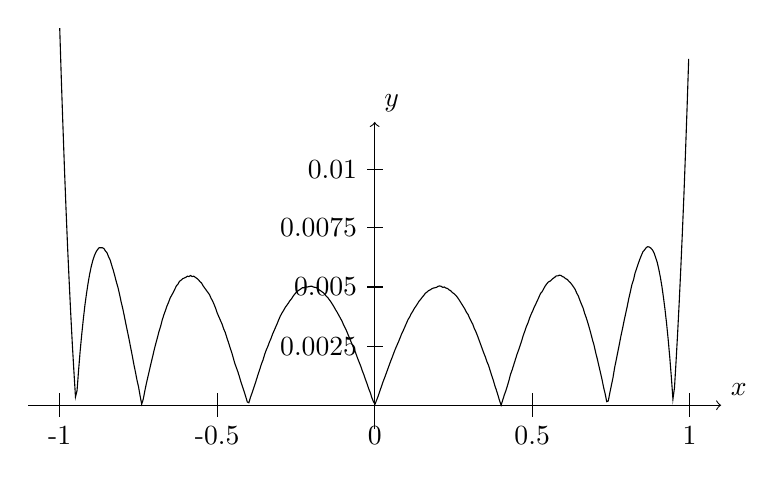
\begin{tikzpicture}[xscale=4,yscale=300]
\draw[->] (-1.1,0) -- (1.1,0) node [above right] {$x$};
\foreach \x in {-1,-0.5,...,1} \draw (\x,0.0005) -- (\x,-0.0005) node [below] {\x};
\draw[->] (0,-0.001) -- (0,0.012) node [above right] {$y$}; 
\foreach \y in {0.0025,0.005,0.0075,0.01} \draw (0.025,\y) -- (-0.025,\y) node [left] {\y};
\draw plot[domain=-1:1,samples=400] (\x,{abs(sin(pi*\x r)-\x*(3.103460404+(-4.814388214+1.726905092*pow(\x,2))*pow(\x,2)))});
\end{tikzpicture}
\end{center}


\end{example}

This last example shows the power of projections.  If we are using functions as elements of vector spaces, then a projection of a function onto a vector space (using the span of a vector space), is the closest function in the vector space to the original function.  In Chapter \ref{ch:fourier:series}, we will do this with trigonometric function and is called Fourier Series. 

%In general this applies to any inner product space.  We can take any point (thought of as a point vector) in the space and project it onto a subspace.  The resulting vector (thought of also as a point) is the point in the subspace closest to the original point. The term closest requires a distance, which is the norm as explained in the following theorem. 
%
%\begin{theorem}
%Consider $S$ a subspace of $\mathbb{R}^n$.  If $\vec{s} \in S$, then, for any $\vec{x} \in \mathbb{R}^2$ then the $\vec{s}$ that satisfies
%%
%\begin{align*}
%\min_{\vec{s} \in S} ||\vec{x}-\vec{s}|| 
%\end{align*}
%is given by 
%%
%\begin{align*}
%\vec{s} = \text{proj}_S \vec{x}
%\end{align*}
%\end{theorem}
%
%\begin{proof}
%Let $E$ be the square of the norm that represents the distance between the point $\vec{x}$ and any $\vec{s} \in S$.  
%
%\begin{align*}
%E(\vec{s}) & = || \vec{s} - \vec{x}|| = \langle \vec{s}-\vec{x},\vec{s} - \vec{x} \rangle \\
%& = \langle \vec{s},\vec{s} \rangle - 2 \langle \vec{x},\vec{s}\rangle + \langle \vec{x}, \vec{x} \rangle 
%\end{align*}
%If we differentiate $E$ with respect to $\vec{s}$, then the result is:
%%
%\begin{align*}
%\frac{\partial E}{\partial \vec{s}} &  = 2 \vec{s} - 
%\end{align*}
%
%{\color{red} ARRGGGG!!  Maybe write as a projection matrix first.  }  
%\end{proof}
%


%\subsection{Projection Matrices}
%
%Since from Theorem \ref{thm:proj:map}, that the projection map is a linear transformation and from Theorem \ref{thm:linear:trans:matrix} that a linear transformation, we examine the projection map as a matrix.  Let's first consider the projection of 
%
%{\color{red} Not sure what I want to do here.}  
%
%\begin{example}
% The transformation matrices for the previous theorems are:
% 
%\begin{enumerate}
% 
%\item 
% % 
%\begin{align*}
%\begin{bmatrix}
% 1 & 0 \\ 0 & -1 
%\end{bmatrix}
%\end{align*}
%
%\item 
%\begin{align*}
%\begin{bmatrix}
% \cos \theta & -\sin \theta \\ \sin \theta & \cos \theta 
%\end{bmatrix}
%\end{align*}
%
%\item To show that the projection operation above can be written as a matrix, let $\vec{v} = [v_1,v_2,v_3]^T$ and write:
%% 
%\begin{align*}
% P \vec{v} & = A_T \vec{v}  = 
%\begin{bmatrix}
% a_{11} & a_{12} & a_{13} \\
% a_{21} & a_{22} & a_{23} \\
% a_{31} & a_{32} & a_{33} \\
%\end{bmatrix} 
%\begin{bmatrix}
% v_1 \\ v_2 \\v_3 
%\end{bmatrix}  = 
%\begin{bmatrix}
% a_{11} v_1 + a_{12} v_2 + a_{13} v_3 \\
% a_{21} v_1 + a_{22} v_2 + a_{23} v_3 \\
% a_{31} v_1 + a_{32} v_2 + a_{33} v_3 \\
%\end{bmatrix}
%\\
%&  = 
%\begin{bmatrix}
% v_1 \\ v_2 \\v_3 
%\end{bmatrix}^T  
%\frac{1}{\sqrt{10}} 
%\begin{bmatrix}
% 3 \\ 0 \\ -1 
%\end{bmatrix}\frac{1}{\sqrt{10}} 
%\begin{bmatrix}
% 3 \\ 0 \\ -1 
%\end{bmatrix} + 
%\begin{bmatrix}
% v_1 \\ v_2 \\v_3 
%\end{bmatrix}^T \frac{1}{\sqrt{35}} 
%\begin{bmatrix}
% 1 \\ -5 \\ 3 
%\end{bmatrix} \frac{1}{\sqrt{35}} 
%\begin{bmatrix}
% 1 \\ -5 \\ 3 
%\end{bmatrix} \\
%& = \frac{1}{10} (3 v_1 -v_3) 
%\begin{bmatrix}
% 3 \\ 0 \\ -1 
%\end{bmatrix} + \frac{1}{35} (v_1 - 5v_2 + 3v_3) 
%\begin{bmatrix}
% 1 \\ -5 \\ 3 
%\end{bmatrix} \\
%& = 
%\begin{bmatrix}
% (9/10 + 1/35)  v_1 - 1/7 v_2 + (3/35-3/10) v_3 \\
% -1/7 v_1 + 5/7 v_2 -3/7 v_3 \\
% (3/10+3/35) v_1 -3/7 v_2 + (1/10 +9/35)v_3 
%\end{bmatrix}  \\ & =
%\begin{bmatrix}
%13/14 & -1/7 & -3/14 \\
% -1/7 & 5/7 & -3/7 \\
%-3/14 & -3/7 & 5/14
%\end{bmatrix} 
%\begin{bmatrix}
% v_1 \\ v_2 \\ v_3  
%\end{bmatrix}
%\end{align*}
%\end{enumerate}
%\end{example}
